%
% db2.tex -- daubechies wavelet 2
%
% (c) 2019 Prof Dr Andreas Müller, Hochschule Rapperswil
%
\documentclass[tikz]{standalone}
\usepackage{amsmath}
\usepackage{times}
\usepackage{txfonts}
\usepackage{pgfplots}
\usepackage{csvsimple}
\usetikzlibrary{arrows,intersections,math}
\begin{document}
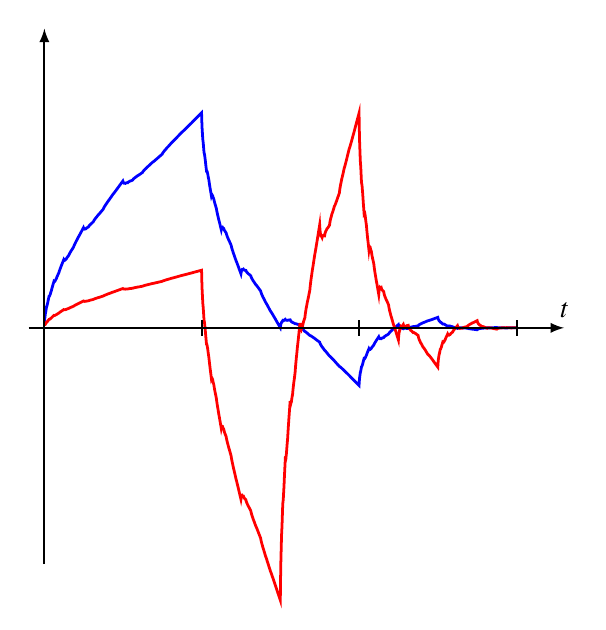
\begin{tikzpicture}[>=latex,scale=2]

\draw[line width=1pt,color=blue] (0.00000, 0.03235)
--(0.00195, 0.05603)
--(0.00391, 0.07104)
--(0.00586, 0.08838)
--(0.00781, 0.09705)
--(0.00977, 0.10804)
--(0.01172, 0.12135)
--(0.01367, 0.13404)
--(0.01562, 0.13806)
--(0.01758, 0.14441)
--(0.01953, 0.15308)
--(0.02148, 0.16112)
--(0.02344, 0.17149)
--(0.02539, 0.18124)
--(0.02734, 0.19036)
--(0.02930, 0.19965)
--(0.03125, 0.20027)
--(0.03320, 0.20322)
--(0.03516, 0.20848)
--(0.03711, 0.21313)
--(0.03906, 0.22010)
--(0.04102, 0.22644)
--(0.04297, 0.23217)
--(0.04492, 0.23805)
--(0.04688, 0.24627)
--(0.04883, 0.25386)
--(0.05078, 0.26082)
--(0.05273, 0.26796)
--(0.05469, 0.27447)
--(0.05664, 0.28115)
--(0.05859, 0.28800)
--(0.06055, 0.29480)
--(0.06250, 0.29293)
--(0.06445, 0.29338)
--(0.06641, 0.29616)
--(0.06836, 0.29832)
--(0.07031, 0.30280)
--(0.07227, 0.30665)
--(0.07422, 0.30989)
--(0.07617, 0.31329)
--(0.07812, 0.31901)
--(0.08008, 0.32411)
--(0.08203, 0.32859)
--(0.08398, 0.33323)
--(0.08594, 0.33726)
--(0.08789, 0.34145)
--(0.08984, 0.34580)
--(0.09180, 0.35011)
--(0.09375, 0.35675)
--(0.09570, 0.36276)
--(0.09766, 0.36815)
--(0.09961, 0.37371)
--(0.10156, 0.37864)
--(0.10352, 0.38374)
--(0.10547, 0.38901)
--(0.10742, 0.39423)
--(0.10938, 0.39883)
--(0.11133, 0.40360)
--(0.11328, 0.40853)
--(0.11523, 0.41342)
--(0.11719, 0.41848)
--(0.11914, 0.42349)
--(0.12109, 0.42846)
--(0.12305, 0.43343)
--(0.12500, 0.42974)
--(0.12695, 0.42838)
--(0.12891, 0.42933)
--(0.13086, 0.42967)
--(0.13281, 0.43232)
--(0.13477, 0.43436)
--(0.13672, 0.43577)
--(0.13867, 0.43735)
--(0.14062, 0.44125)
--(0.14258, 0.44453)
--(0.14453, 0.44718)
--(0.14648, 0.45000)
--(0.14844, 0.45221)
--(0.15039, 0.45457)
--(0.15234, 0.45711)
--(0.15430, 0.45960)
--(0.15625, 0.46441)
--(0.15820, 0.46860)
--(0.16016, 0.47216)
--(0.16211, 0.47590)
--(0.16406, 0.47901)
--(0.16602, 0.48229)
--(0.16797, 0.48573)
--(0.16992, 0.48913)
--(0.17188, 0.49191)
--(0.17383, 0.49486)
--(0.17578, 0.49797)
--(0.17773, 0.50104)
--(0.17969, 0.50427)
--(0.18164, 0.50746)
--(0.18359, 0.51060)
--(0.18555, 0.51376)
--(0.18750, 0.51924)
--(0.18945, 0.52409)
--(0.19141, 0.52833)
--(0.19336, 0.53273)
--(0.19531, 0.53651)
--(0.19727, 0.54045)
--(0.19922, 0.54457)
--(0.20117, 0.54863)
--(0.20312, 0.55208)
--(0.20508, 0.55569)
--(0.20703, 0.55947)
--(0.20898, 0.56320)
--(0.21094, 0.56710)
--(0.21289, 0.57096)
--(0.21484, 0.57477)
--(0.21680, 0.57859)
--(0.21875, 0.58179)
--(0.22070, 0.58516)
--(0.22266, 0.58870)
--(0.22461, 0.59219)
--(0.22656, 0.59584)
--(0.22852, 0.59945)
--(0.23047, 0.60302)
--(0.23242, 0.60660)
--(0.23438, 0.61035)
--(0.23633, 0.61405)
--(0.23828, 0.61770)
--(0.24023, 0.62137)
--(0.24219, 0.62500)
--(0.24414, 0.62863)
--(0.24609, 0.63228)
--(0.24805, 0.63593)
--(0.25000, 0.63090)
--(0.25195, 0.62820)
--(0.25391, 0.62782)
--(0.25586, 0.62682)
--(0.25781, 0.62814)
--(0.25977, 0.62884)
--(0.26172, 0.62892)
--(0.26367, 0.62917)
--(0.26562, 0.63173)
--(0.26758, 0.63368)
--(0.26953, 0.63500)
--(0.27148, 0.63649)
--(0.27344, 0.63735)
--(0.27539, 0.63839)
--(0.27734, 0.63959)
--(0.27930, 0.64074)
--(0.28125, 0.64422)
--(0.28320, 0.64708)
--(0.28516, 0.64931)
--(0.28711, 0.65171)
--(0.28906, 0.65349)
--(0.29102, 0.65543)
--(0.29297, 0.65754)
--(0.29492, 0.65961)
--(0.29688, 0.66105)
--(0.29883, 0.66266)
--(0.30078, 0.66444)
--(0.30273, 0.66617)
--(0.30469, 0.66807)
--(0.30664, 0.66993)
--(0.30859, 0.67174)
--(0.31055, 0.67356)
--(0.31250, 0.67771)
--(0.31445, 0.68123)
--(0.31641, 0.68413)
--(0.31836, 0.68720)
--(0.32031, 0.68964)
--(0.32227, 0.69225)
--(0.32422, 0.69503)
--(0.32617, 0.69776)
--(0.32812, 0.69987)
--(0.33008, 0.70215)
--(0.33203, 0.70460)
--(0.33398, 0.70700)
--(0.33594, 0.70956)
--(0.33789, 0.71209)
--(0.33984, 0.71456)
--(0.34180, 0.71705)
--(0.34375, 0.71892)
--(0.34570, 0.72095)
--(0.34766, 0.72315)
--(0.34961, 0.72531)
--(0.35156, 0.72763)
--(0.35352, 0.72991)
--(0.35547, 0.73214)
--(0.35742, 0.73439)
--(0.35938, 0.73680)
--(0.36133, 0.73917)
--(0.36328, 0.74149)
--(0.36523, 0.74382)
--(0.36719, 0.74611)
--(0.36914, 0.74842)
--(0.37109, 0.75073)
--(0.37305, 0.75304)
--(0.37500, 0.75767)
--(0.37695, 0.76168)
--(0.37891, 0.76507)
--(0.38086, 0.76863)
--(0.38281, 0.77156)
--(0.38477, 0.77466)
--(0.38672, 0.77793)
--(0.38867, 0.78115)
--(0.39062, 0.78375)
--(0.39258, 0.78651)
--(0.39453, 0.78945)
--(0.39648, 0.79234)
--(0.39844, 0.79539)
--(0.40039, 0.79840)
--(0.40234, 0.80137)
--(0.40430, 0.80434)
--(0.40625, 0.80670)
--(0.40820, 0.80922)
--(0.41016, 0.81191)
--(0.41211, 0.81455)
--(0.41406, 0.81736)
--(0.41602, 0.82013)
--(0.41797, 0.82285)
--(0.41992, 0.82559)
--(0.42188, 0.82849)
--(0.42383, 0.83134)
--(0.42578, 0.83415)
--(0.42773, 0.83697)
--(0.42969, 0.83975)
--(0.43164, 0.84254)
--(0.43359, 0.84535)
--(0.43555, 0.84814)
--(0.43750, 0.85032)
--(0.43945, 0.85266)
--(0.44141, 0.85517)
--(0.44336, 0.85764)
--(0.44531, 0.86027)
--(0.44727, 0.86286)
--(0.44922, 0.86540)
--(0.45117, 0.86796)
--(0.45312, 0.87068)
--(0.45508, 0.87335)
--(0.45703, 0.87599)
--(0.45898, 0.87863)
--(0.46094, 0.88123)
--(0.46289, 0.88384)
--(0.46484, 0.88646)
--(0.46680, 0.88908)
--(0.46875, 0.89187)
--(0.47070, 0.89461)
--(0.47266, 0.89731)
--(0.47461, 0.90002)
--(0.47656, 0.90269)
--(0.47852, 0.90536)
--(0.48047, 0.90805)
--(0.48242, 0.91074)
--(0.48438, 0.91338)
--(0.48633, 0.91603)
--(0.48828, 0.91870)
--(0.49023, 0.92136)
--(0.49219, 0.92403)
--(0.49414, 0.92670)
--(0.49609, 0.92937)
--(0.49805, 0.93204)
--(0.50000, 0.92604)
--(0.50195, 0.92236)
--(0.50391, 0.92100)
--(0.50586, 0.91903)
--(0.50781, 0.91937)
--(0.50977, 0.91910)
--(0.51172, 0.91820)
--(0.51367, 0.91746)
--(0.51562, 0.91905)
--(0.51758, 0.92002)
--(0.51953, 0.92037)
--(0.52148, 0.92088)
--(0.52344, 0.92077)
--(0.52539, 0.92083)
--(0.52734, 0.92105)
--(0.52930, 0.92123)
--(0.53125, 0.92373)
--(0.53320, 0.92561)
--(0.53516, 0.92687)
--(0.53711, 0.92829)
--(0.53906, 0.92909)
--(0.54102, 0.93006)
--(0.54297, 0.93119)
--(0.54492, 0.93228)
--(0.54688, 0.93275)
--(0.54883, 0.93338)
--(0.55078, 0.93418)
--(0.55273, 0.93494)
--(0.55469, 0.93586)
--(0.55664, 0.93674)
--(0.55859, 0.93758)
--(0.56055, 0.93842)
--(0.56250, 0.94159)
--(0.56445, 0.94414)
--(0.56641, 0.94606)
--(0.56836, 0.94815)
--(0.57031, 0.94962)
--(0.57227, 0.95125)
--(0.57422, 0.95305)
--(0.57617, 0.95481)
--(0.57812, 0.95595)
--(0.58008, 0.95725)
--(0.58203, 0.95872)
--(0.58398, 0.96014)
--(0.58594, 0.96173)
--(0.58789, 0.96327)
--(0.58984, 0.96478)
--(0.59180, 0.96629)
--(0.59375, 0.96718)
--(0.59570, 0.96824)
--(0.59766, 0.96946)
--(0.59961, 0.97064)
--(0.60156, 0.97198)
--(0.60352, 0.97329)
--(0.60547, 0.97454)
--(0.60742, 0.97581)
--(0.60938, 0.97725)
--(0.61133, 0.97864)
--(0.61328, 0.97998)
--(0.61523, 0.98134)
--(0.61719, 0.98265)
--(0.61914, 0.98398)
--(0.62109, 0.98532)
--(0.62305, 0.98665)
--(0.62500, 0.99031)
--(0.62695, 0.99334)
--(0.62891, 0.99575)
--(0.63086, 0.99833)
--(0.63281, 1.00029)
--(0.63477, 1.00241)
--(0.63672, 1.00470)
--(0.63867, 1.00695)
--(0.64062, 1.00857)
--(0.64258, 1.01036)
--(0.64453, 1.01232)
--(0.64648, 1.01423)
--(0.64844, 1.01631)
--(0.65039, 1.01834)
--(0.65234, 1.02033)
--(0.65430, 1.02233)
--(0.65625, 1.02371)
--(0.65820, 1.02525)
--(0.66016, 1.02697)
--(0.66211, 1.02863)
--(0.66406, 1.03047)
--(0.66602, 1.03226)
--(0.66797, 1.03400)
--(0.66992, 1.03576)
--(0.67188, 1.03768)
--(0.67383, 1.03956)
--(0.67578, 1.04140)
--(0.67773, 1.04324)
--(0.67969, 1.04504)
--(0.68164, 1.04686)
--(0.68359, 1.04868)
--(0.68555, 1.05050)
--(0.68750, 1.05170)
--(0.68945, 1.05307)
--(0.69141, 1.05460)
--(0.69336, 1.05609)
--(0.69531, 1.05775)
--(0.69727, 1.05936)
--(0.69922, 1.06093)
--(0.70117, 1.06250)
--(0.70312, 1.06425)
--(0.70508, 1.06595)
--(0.70703, 1.06761)
--(0.70898, 1.06927)
--(0.71094, 1.07090)
--(0.71289, 1.07253)
--(0.71484, 1.07418)
--(0.71680, 1.07582)
--(0.71875, 1.07763)
--(0.72070, 1.07940)
--(0.72266, 1.08112)
--(0.72461, 1.08285)
--(0.72656, 1.08454)
--(0.72852, 1.08624)
--(0.73047, 1.08795)
--(0.73242, 1.08966)
--(0.73438, 1.09132)
--(0.73633, 1.09300)
--(0.73828, 1.09469)
--(0.74023, 1.09637)
--(0.74219, 1.09807)
--(0.74414, 1.09976)
--(0.74609, 1.10146)
--(0.74805, 1.10315)
--(0.75000, 1.10716)
--(0.75195, 1.11055)
--(0.75391, 1.11332)
--(0.75586, 1.11626)
--(0.75781, 1.11857)
--(0.75977, 1.12105)
--(0.76172, 1.12370)
--(0.76367, 1.12630)
--(0.76562, 1.12828)
--(0.76758, 1.13043)
--(0.76953, 1.13274)
--(0.77148, 1.13501)
--(0.77344, 1.13745)
--(0.77539, 1.13984)
--(0.77734, 1.14219)
--(0.77930, 1.14454)
--(0.78125, 1.14628)
--(0.78320, 1.14818)
--(0.78516, 1.15025)
--(0.78711, 1.15228)
--(0.78906, 1.15447)
--(0.79102, 1.15662)
--(0.79297, 1.15872)
--(0.79492, 1.16083)
--(0.79688, 1.16311)
--(0.79883, 1.16535)
--(0.80078, 1.16754)
--(0.80273, 1.16975)
--(0.80469, 1.17191)
--(0.80664, 1.17408)
--(0.80859, 1.17626)
--(0.81055, 1.17844)
--(0.81250, 1.18000)
--(0.81445, 1.18172)
--(0.81641, 1.18361)
--(0.81836, 1.18546)
--(0.82031, 1.18747)
--(0.82227, 1.18944)
--(0.82422, 1.19136)
--(0.82617, 1.19330)
--(0.82812, 1.19540)
--(0.83008, 1.19746)
--(0.83203, 1.19947)
--(0.83398, 1.20150)
--(0.83594, 1.20348)
--(0.83789, 1.20547)
--(0.83984, 1.20747)
--(0.84180, 1.20947)
--(0.84375, 1.21164)
--(0.84570, 1.21376)
--(0.84766, 1.21584)
--(0.84961, 1.21793)
--(0.85156, 1.21998)
--(0.85352, 1.22204)
--(0.85547, 1.22411)
--(0.85742, 1.22617)
--(0.85938, 1.22819)
--(0.86133, 1.23023)
--(0.86328, 1.23227)
--(0.86523, 1.23432)
--(0.86719, 1.23637)
--(0.86914, 1.23842)
--(0.87109, 1.24047)
--(0.87305, 1.24252)
--(0.87500, 1.24395)
--(0.87695, 1.24554)
--(0.87891, 1.24730)
--(0.88086, 1.24901)
--(0.88281, 1.25090)
--(0.88477, 1.25273)
--(0.88672, 1.25453)
--(0.88867, 1.25633)
--(0.89062, 1.25830)
--(0.89258, 1.26023)
--(0.89453, 1.26211)
--(0.89648, 1.26401)
--(0.89844, 1.26586)
--(0.90039, 1.26772)
--(0.90234, 1.26959)
--(0.90430, 1.27146)
--(0.90625, 1.27350)
--(0.90820, 1.27549)
--(0.91016, 1.27744)
--(0.91211, 1.27940)
--(0.91406, 1.28131)
--(0.91602, 1.28324)
--(0.91797, 1.28518)
--(0.91992, 1.28711)
--(0.92188, 1.28900)
--(0.92383, 1.29091)
--(0.92578, 1.29282)
--(0.92773, 1.29473)
--(0.92969, 1.29666)
--(0.93164, 1.29858)
--(0.93359, 1.30049)
--(0.93555, 1.30241)
--(0.93750, 1.30450)
--(0.93945, 1.30654)
--(0.94141, 1.30853)
--(0.94336, 1.31054)
--(0.94531, 1.31250)
--(0.94727, 1.31448)
--(0.94922, 1.31646)
--(0.95117, 1.31845)
--(0.95312, 1.32039)
--(0.95508, 1.32234)
--(0.95703, 1.32430)
--(0.95898, 1.32626)
--(0.96094, 1.32823)
--(0.96289, 1.33020)
--(0.96484, 1.33217)
--(0.96680, 1.33413)
--(0.96875, 1.33605)
--(0.97070, 1.33799)
--(0.97266, 1.33993)
--(0.97461, 1.34187)
--(0.97656, 1.34383)
--(0.97852, 1.34578)
--(0.98047, 1.34773)
--(0.98242, 1.34967)
--(0.98438, 1.35163)
--(0.98633, 1.35359)
--(0.98828, 1.35555)
--(0.99023, 1.35750)
--(0.99219, 1.35945)
--(0.99414, 1.36140)
--(0.99609, 1.36336)
--(0.99805, 1.36531)
--(1.00000, 1.30257)
--(1.00195, 1.25716)
--(1.00391, 1.22908)
--(1.00586, 1.19637)
--(1.00781, 1.18098)
--(1.00977, 1.16096)
--(1.01172, 1.13628)
--(1.01367, 1.11285)
--(1.01562, 1.10676)
--(1.01758, 1.09602)
--(1.01953, 1.08064)
--(1.02148, 1.06650)
--(1.02344, 1.04772)
--(1.02539, 1.03018)
--(1.02734, 1.01389)
--(1.02930, 0.99726)
--(1.03125, 0.99797)
--(1.03320, 0.99403)
--(1.03516, 0.98545)
--(1.03711, 0.97811)
--(1.03906, 0.96613)
--(1.04102, 0.95540)
--(1.04297, 0.94590)
--(1.04492, 0.93608)
--(1.04688, 0.92160)
--(1.04883, 0.90838)
--(1.05078, 0.89640)
--(1.05273, 0.88408)
--(1.05469, 0.87301)
--(1.05664, 0.86160)
--(1.05859, 0.84987)
--(1.06055, 0.83822)
--(1.06250, 0.84390)
--(1.06445, 0.84495)
--(1.06641, 0.84134)
--(1.06836, 0.83899)
--(1.07031, 0.83198)
--(1.07227, 0.82622)
--(1.07422, 0.82171)
--(1.07617, 0.81686)
--(1.07812, 0.80737)
--(1.08008, 0.79912)
--(1.08203, 0.79212)
--(1.08398, 0.78478)
--(1.08594, 0.77869)
--(1.08789, 0.77226)
--(1.08984, 0.76550)
--(1.09180, 0.75883)
--(1.09375, 0.74752)
--(1.09570, 0.73745)
--(1.09766, 0.72862)
--(1.09961, 0.71946)
--(1.10156, 0.71155)
--(1.10352, 0.70330)
--(1.10547, 0.69472)
--(1.10742, 0.68622)
--(1.10938, 0.67898)
--(1.11133, 0.67139)
--(1.11328, 0.66348)
--(1.11523, 0.65565)
--(1.11719, 0.64750)
--(1.11914, 0.63943)
--(1.12109, 0.63145)
--(1.12305, 0.62344)
--(1.12500, 0.63277)
--(1.12695, 0.63746)
--(1.12891, 0.63750)
--(1.13086, 0.63879)
--(1.13281, 0.63543)
--(1.13477, 0.63331)
--(1.13672, 0.63245)
--(1.13867, 0.63124)
--(1.14062, 0.62539)
--(1.14258, 0.62079)
--(1.14453, 0.61743)
--(1.14648, 0.61374)
--(1.14844, 0.61129)
--(1.15039, 0.60851)
--(1.15234, 0.60539)
--(1.15430, 0.60237)
--(1.15625, 0.59470)
--(1.15820, 0.58827)
--(1.16016, 0.58309)
--(1.16211, 0.57758)
--(1.16406, 0.57331)
--(1.16602, 0.56870)
--(1.16797, 0.56377)
--(1.16992, 0.55892)
--(1.17188, 0.55532)
--(1.17383, 0.55138)
--(1.17578, 0.54711)
--(1.17773, 0.54293)
--(1.17969, 0.53841)
--(1.18164, 0.53399)
--(1.18359, 0.52965)
--(1.18555, 0.52529)
--(1.18750, 0.51629)
--(1.18945, 0.50853)
--(1.19141, 0.50201)
--(1.19336, 0.49516)
--(1.19531, 0.48956)
--(1.19727, 0.48362)
--(1.19922, 0.47735)
--(1.20117, 0.47117)
--(1.20312, 0.46623)
--(1.20508, 0.46096)
--(1.20703, 0.45536)
--(1.20898, 0.44984)
--(1.21094, 0.44400)
--(1.21289, 0.43824)
--(1.21484, 0.43257)
--(1.21680, 0.42687)
--(1.21875, 0.42242)
--(1.22070, 0.41764)
--(1.22266, 0.41253)
--(1.22461, 0.40750)
--(1.22656, 0.40214)
--(1.22852, 0.39687)
--(1.23047, 0.39169)
--(1.23242, 0.38648)
--(1.23438, 0.38094)
--(1.23633, 0.37549)
--(1.23828, 0.37013)
--(1.24023, 0.36475)
--(1.24219, 0.35946)
--(1.24414, 0.35414)
--(1.24609, 0.34880)
--(1.24805, 0.34346)
--(1.25000, 0.35546)
--(1.25195, 0.36281)
--(1.25391, 0.36552)
--(1.25586, 0.36948)
--(1.25781, 0.36879)
--(1.25977, 0.36934)
--(1.26172, 0.37114)
--(1.26367, 0.37260)
--(1.26562, 0.36942)
--(1.26758, 0.36749)
--(1.26953, 0.36680)
--(1.27148, 0.36577)
--(1.27344, 0.36599)
--(1.27539, 0.36588)
--(1.27734, 0.36543)
--(1.27930, 0.36507)
--(1.28125, 0.36007)
--(1.28320, 0.35631)
--(1.28516, 0.35380)
--(1.28711, 0.35095)
--(1.28906, 0.34935)
--(1.29102, 0.34742)
--(1.29297, 0.34515)
--(1.29492, 0.34297)
--(1.29688, 0.34203)
--(1.29883, 0.34076)
--(1.30078, 0.33916)
--(1.30273, 0.33765)
--(1.30469, 0.33580)
--(1.30664, 0.33405)
--(1.30859, 0.33238)
--(1.31055, 0.33069)
--(1.31250, 0.32435)
--(1.31445, 0.31926)
--(1.31641, 0.31541)
--(1.31836, 0.31123)
--(1.32031, 0.30829)
--(1.32227, 0.30503)
--(1.32422, 0.30142)
--(1.32617, 0.29791)
--(1.32812, 0.29564)
--(1.33008, 0.29304)
--(1.33203, 0.29010)
--(1.33398, 0.28725)
--(1.33594, 0.28407)
--(1.33789, 0.28098)
--(1.33984, 0.27798)
--(1.34180, 0.27496)
--(1.34375, 0.27317)
--(1.34570, 0.27106)
--(1.34766, 0.26861)
--(1.34961, 0.26625)
--(1.35156, 0.26356)
--(1.35352, 0.26096)
--(1.35547, 0.25845)
--(1.35742, 0.25591)
--(1.35938, 0.25304)
--(1.36133, 0.25026)
--(1.36328, 0.24757)
--(1.36523, 0.24485)
--(1.36719, 0.24222)
--(1.36914, 0.23957)
--(1.37109, 0.23690)
--(1.37305, 0.23423)
--(1.37500, 0.22692)
--(1.37695, 0.22085)
--(1.37891, 0.21602)
--(1.38086, 0.21087)
--(1.38281, 0.20695)
--(1.38477, 0.20271)
--(1.38672, 0.19813)
--(1.38867, 0.19364)
--(1.39062, 0.19039)
--(1.39258, 0.18681)
--(1.39453, 0.18290)
--(1.39648, 0.17908)
--(1.39844, 0.17492)
--(1.40039, 0.17085)
--(1.40234, 0.16688)
--(1.40430, 0.16287)
--(1.40625, 0.16012)
--(1.40820, 0.15702)
--(1.41016, 0.15360)
--(1.41211, 0.15027)
--(1.41406, 0.14660)
--(1.41602, 0.14302)
--(1.41797, 0.13953)
--(1.41992, 0.13601)
--(1.42188, 0.13217)
--(1.42383, 0.12841)
--(1.42578, 0.12474)
--(1.42773, 0.12105)
--(1.42969, 0.11744)
--(1.43164, 0.11382)
--(1.43359, 0.11017)
--(1.43555, 0.10652)
--(1.43750, 0.10412)
--(1.43945, 0.10139)
--(1.44141, 0.09832)
--(1.44336, 0.09534)
--(1.44531, 0.09203)
--(1.44727, 0.08881)
--(1.44922, 0.08568)
--(1.45117, 0.08252)
--(1.45312, 0.07903)
--(1.45508, 0.07563)
--(1.45703, 0.07232)
--(1.45898, 0.06899)
--(1.46094, 0.06574)
--(1.46289, 0.06247)
--(1.46484, 0.05918)
--(1.46680, 0.05589)
--(1.46875, 0.05227)
--(1.47070, 0.04874)
--(1.47266, 0.04530)
--(1.47461, 0.04183)
--(1.47656, 0.03845)
--(1.47852, 0.03505)
--(1.48047, 0.03163)
--(1.48242, 0.02821)
--(1.48438, 0.02488)
--(1.48633, 0.02153)
--(1.48828, 0.01815)
--(1.49023, 0.01478)
--(1.49219, 0.01139)
--(1.49414, 0.00800)
--(1.49609, 0.00462)
--(1.49805, 0.00124)
--(1.50000, 0.01519)
--(1.50195, 0.02450)
--(1.50391, 0.02916)
--(1.50586, 0.03507)
--(1.50781, 0.03633)
--(1.50977, 0.03884)
--(1.51172, 0.04259)
--(1.51367, 0.04601)
--(1.51562, 0.04478)
--(1.51758, 0.04480)
--(1.51953, 0.04606)
--(1.52148, 0.04699)
--(1.52344, 0.04916)
--(1.52539, 0.05100)
--(1.52734, 0.05251)
--(1.52930, 0.05410)
--(1.53125, 0.05105)
--(1.53320, 0.04925)
--(1.53516, 0.04869)
--(1.53711, 0.04780)
--(1.53906, 0.04815)
--(1.54102, 0.04816)
--(1.54297, 0.04785)
--(1.54492, 0.04762)
--(1.54688, 0.04864)
--(1.54883, 0.04932)
--(1.55078, 0.04968)
--(1.55273, 0.05012)
--(1.55469, 0.05022)
--(1.55664, 0.05042)
--(1.55859, 0.05070)
--(1.56055, 0.05097)
--(1.56250, 0.04658)
--(1.56445, 0.04344)
--(1.56641, 0.04155)
--(1.56836, 0.03932)
--(1.57031, 0.03834)
--(1.57227, 0.03702)
--(1.57422, 0.03537)
--(1.57617, 0.03381)
--(1.57812, 0.03350)
--(1.58008, 0.03285)
--(1.58203, 0.03186)
--(1.58398, 0.03097)
--(1.58594, 0.02974)
--(1.58789, 0.02861)
--(1.58984, 0.02756)
--(1.59180, 0.02648)
--(1.59375, 0.02666)
--(1.59570, 0.02650)
--(1.59766, 0.02600)
--(1.59961, 0.02560)
--(1.60156, 0.02486)
--(1.60352, 0.02421)
--(1.60547, 0.02365)
--(1.60742, 0.02306)
--(1.60938, 0.02215)
--(1.61133, 0.02132)
--(1.61328, 0.02058)
--(1.61523, 0.01982)
--(1.61719, 0.01914)
--(1.61914, 0.01844)
--(1.62109, 0.01772)
--(1.62305, 0.01701)
--(1.62500, 0.01165)
--(1.62695, 0.00753)
--(1.62891, 0.00466)
--(1.63086, 0.00146)
--(1.63281, -0.00050)
--(1.63477, -0.00279)
--(1.63672, -0.00542)
--(1.63867, -0.00796)
--(1.64062, -0.00925)
--(1.64258, -0.01088)
--(1.64453, -0.01284)
--(1.64648, -0.01471)
--(1.64844, -0.01691)
--(1.65039, -0.01902)
--(1.65234, -0.02105)
--(1.65430, -0.02310)
--(1.65625, -0.02390)
--(1.65820, -0.02504)
--(1.66016, -0.02651)
--(1.66211, -0.02789)
--(1.66406, -0.02961)
--(1.66602, -0.03123)
--(1.66797, -0.03277)
--(1.66992, -0.03433)
--(1.67188, -0.03623)
--(1.67383, -0.03803)
--(1.67578, -0.03975)
--(1.67773, -0.04149)
--(1.67969, -0.04314)
--(1.68164, -0.04481)
--(1.68359, -0.04651)
--(1.68555, -0.04820)
--(1.68750, -0.04865)
--(1.68945, -0.04943)
--(1.69141, -0.05054)
--(1.69336, -0.05156)
--(1.69531, -0.05292)
--(1.69727, -0.05419)
--(1.69922, -0.05537)
--(1.70117, -0.05657)
--(1.70312, -0.05811)
--(1.70508, -0.05956)
--(1.70703, -0.06092)
--(1.70898, -0.06230)
--(1.71094, -0.06359)
--(1.71289, -0.06491)
--(1.71484, -0.06625)
--(1.71680, -0.06758)
--(1.71875, -0.06925)
--(1.72070, -0.07083)
--(1.72266, -0.07232)
--(1.72461, -0.07383)
--(1.72656, -0.07525)
--(1.72852, -0.07670)
--(1.73047, -0.07817)
--(1.73242, -0.07963)
--(1.73438, -0.08101)
--(1.73633, -0.08241)
--(1.73828, -0.08383)
--(1.74023, -0.08525)
--(1.74219, -0.08669)
--(1.74414, -0.08813)
--(1.74609, -0.08955)
--(1.74805, -0.09098)
--(1.75000, -0.09706)
--(1.75195, -0.10189)
--(1.75391, -0.10547)
--(1.75586, -0.10939)
--(1.75781, -0.11207)
--(1.75977, -0.11508)
--(1.76172, -0.11842)
--(1.76367, -0.12167)
--(1.76562, -0.12368)
--(1.76758, -0.12602)
--(1.76953, -0.12869)
--(1.77148, -0.13128)
--(1.77344, -0.13420)
--(1.77539, -0.13702)
--(1.77734, -0.13976)
--(1.77930, -0.14253)
--(1.78125, -0.14405)
--(1.78320, -0.14590)
--(1.78516, -0.14809)
--(1.78711, -0.15018)
--(1.78906, -0.15261)
--(1.79102, -0.15495)
--(1.79297, -0.15721)
--(1.79492, -0.15948)
--(1.79688, -0.16209)
--(1.79883, -0.16461)
--(1.80078, -0.16704)
--(1.80273, -0.16949)
--(1.80469, -0.17186)
--(1.80664, -0.17425)
--(1.80859, -0.17666)
--(1.81055, -0.17907)
--(1.81250, -0.18023)
--(1.81445, -0.18172)
--(1.81641, -0.18355)
--(1.81836, -0.18529)
--(1.82031, -0.18736)
--(1.82227, -0.18935)
--(1.82422, -0.19124)
--(1.82617, -0.19316)
--(1.82812, -0.19541)
--(1.83008, -0.19757)
--(1.83203, -0.19965)
--(1.83398, -0.20174)
--(1.83594, -0.20375)
--(1.83789, -0.20578)
--(1.83984, -0.20784)
--(1.84180, -0.20989)
--(1.84375, -0.21227)
--(1.84570, -0.21456)
--(1.84766, -0.21677)
--(1.84961, -0.21899)
--(1.85156, -0.22113)
--(1.85352, -0.22329)
--(1.85547, -0.22548)
--(1.85742, -0.22766)
--(1.85938, -0.22975)
--(1.86133, -0.23186)
--(1.86328, -0.23400)
--(1.86523, -0.23613)
--(1.86719, -0.23829)
--(1.86914, -0.24044)
--(1.87109, -0.24258)
--(1.87305, -0.24473)
--(1.87500, -0.24563)
--(1.87695, -0.24686)
--(1.87891, -0.24843)
--(1.88086, -0.24991)
--(1.88281, -0.25172)
--(1.88477, -0.25344)
--(1.88672, -0.25507)
--(1.88867, -0.25673)
--(1.89062, -0.25872)
--(1.89258, -0.26062)
--(1.89453, -0.26243)
--(1.89648, -0.26426)
--(1.89844, -0.26601)
--(1.90039, -0.26778)
--(1.90234, -0.26957)
--(1.90430, -0.27136)
--(1.90625, -0.27348)
--(1.90820, -0.27551)
--(1.91016, -0.27746)
--(1.91211, -0.27942)
--(1.91406, -0.28130)
--(1.91602, -0.28320)
--(1.91797, -0.28512)
--(1.91992, -0.28704)
--(1.92188, -0.28887)
--(1.92383, -0.29072)
--(1.92578, -0.29260)
--(1.92773, -0.29447)
--(1.92969, -0.29636)
--(1.93164, -0.29825)
--(1.93359, -0.30013)
--(1.93555, -0.30201)
--(1.93750, -0.30423)
--(1.93945, -0.30636)
--(1.94141, -0.30840)
--(1.94336, -0.31046)
--(1.94531, -0.31243)
--(1.94727, -0.31443)
--(1.94922, -0.31645)
--(1.95117, -0.31846)
--(1.95312, -0.32039)
--(1.95508, -0.32233)
--(1.95703, -0.32431)
--(1.95898, -0.32627)
--(1.96094, -0.32826)
--(1.96289, -0.33025)
--(1.96484, -0.33222)
--(1.96680, -0.33420)
--(1.96875, -0.33609)
--(1.97070, -0.33800)
--(1.97266, -0.33994)
--(1.97461, -0.34187)
--(1.97656, -0.34383)
--(1.97852, -0.34578)
--(1.98047, -0.34772)
--(1.98242, -0.34966)
--(1.98438, -0.35163)
--(1.98633, -0.35359)
--(1.98828, -0.35555)
--(1.99023, -0.35750)
--(1.99219, -0.35945)
--(1.99414, -0.36140)
--(1.99609, -0.36336)
--(1.99805, -0.36531)
--(2.00000, -0.33491)
--(2.00195, -0.31319)
--(2.00391, -0.30013)
--(2.00586, -0.28474)
--(2.00781, -0.27803)
--(2.00977, -0.26899)
--(2.01172, -0.25763)
--(2.01367, -0.24689)
--(2.01562, -0.24483)
--(2.01758, -0.24043)
--(2.01953, -0.23372)
--(2.02148, -0.22763)
--(2.02344, -0.21921)
--(2.02539, -0.21142)
--(2.02734, -0.20425)
--(2.02930, -0.19691)
--(2.03125, -0.19824)
--(2.03320, -0.19725)
--(2.03516, -0.19394)
--(2.03711, -0.19124)
--(2.03906, -0.18623)
--(2.04102, -0.18184)
--(2.04297, -0.17807)
--(2.04492, -0.17413)
--(2.04688, -0.16787)
--(2.04883, -0.16223)
--(2.05078, -0.15722)
--(2.05273, -0.15204)
--(2.05469, -0.14748)
--(2.05664, -0.14275)
--(2.05859, -0.13786)
--(2.06055, -0.13301)
--(2.06250, -0.13683)
--(2.06445, -0.13833)
--(2.06641, -0.13751)
--(2.06836, -0.13730)
--(2.07031, -0.13478)
--(2.07227, -0.13288)
--(2.07422, -0.13160)
--(2.07617, -0.13015)
--(2.07812, -0.12638)
--(2.08008, -0.12323)
--(2.08203, -0.12071)
--(2.08398, -0.11801)
--(2.08594, -0.11594)
--(2.08789, -0.11371)
--(2.08984, -0.11130)
--(2.09180, -0.10895)
--(2.09375, -0.10426)
--(2.09570, -0.10021)
--(2.09766, -0.09677)
--(2.09961, -0.09317)
--(2.10156, -0.09019)
--(2.10352, -0.08704)
--(2.10547, -0.08372)
--(2.10742, -0.08045)
--(2.10938, -0.07781)
--(2.11133, -0.07499)
--(2.11328, -0.07201)
--(2.11523, -0.06908)
--(2.11719, -0.06597)
--(2.11914, -0.06292)
--(2.12109, -0.05990)
--(2.12305, -0.05688)
--(2.12500, -0.06252)
--(2.12695, -0.06584)
--(2.12891, -0.06684)
--(2.13086, -0.06846)
--(2.13281, -0.06775)
--(2.13477, -0.06767)
--(2.13672, -0.06821)
--(2.13867, -0.06859)
--(2.14062, -0.06664)
--(2.14258, -0.06532)
--(2.14453, -0.06461)
--(2.14648, -0.06374)
--(2.14844, -0.06350)
--(2.15039, -0.06308)
--(2.15234, -0.06250)
--(2.15430, -0.06196)
--(2.15625, -0.05911)
--(2.15820, -0.05687)
--(2.16016, -0.05526)
--(2.16211, -0.05347)
--(2.16406, -0.05232)
--(2.16602, -0.05099)
--(2.16797, -0.04950)
--(2.16992, -0.04805)
--(2.17188, -0.04723)
--(2.17383, -0.04624)
--(2.17578, -0.04508)
--(2.17773, -0.04396)
--(2.17969, -0.04268)
--(2.18164, -0.04145)
--(2.18359, -0.04026)
--(2.18555, -0.03905)
--(2.18750, -0.03553)
--(2.18945, -0.03262)
--(2.19141, -0.03034)
--(2.19336, -0.02789)
--(2.19531, -0.02607)
--(2.19727, -0.02408)
--(2.19922, -0.02192)
--(2.20117, -0.01980)
--(2.20312, -0.01831)
--(2.20508, -0.01665)
--(2.20703, -0.01483)
--(2.20898, -0.01305)
--(2.21094, -0.01110)
--(2.21289, -0.00920)
--(2.21484, -0.00734)
--(2.21680, -0.00547)
--(2.21875, -0.00422)
--(2.22070, -0.00280)
--(2.22266, -0.00122)
--(2.22461, 0.00031)
--(2.22656, 0.00202)
--(2.22852, 0.00368)
--(2.23047, 0.00529)
--(2.23242, 0.00692)
--(2.23438, 0.00871)
--(2.23633, 0.01046)
--(2.23828, 0.01216)
--(2.24023, 0.01388)
--(2.24219, 0.01555)
--(2.24414, 0.01723)
--(2.24609, 0.01892)
--(2.24805, 0.02062)
--(2.25000, 0.01364)
--(2.25195, 0.00898)
--(2.25391, 0.00665)
--(2.25586, 0.00370)
--(2.25781, 0.00307)
--(2.25977, 0.00182)
--(2.26172, -0.00006)
--(2.26367, -0.00177)
--(2.26562, -0.00116)
--(2.26758, -0.00116)
--(2.26953, -0.00180)
--(2.27148, -0.00226)
--(2.27344, -0.00335)
--(2.27539, -0.00427)
--(2.27734, -0.00502)
--(2.27930, -0.00582)
--(2.28125, -0.00429)
--(2.28320, -0.00339)
--(2.28516, -0.00311)
--(2.28711, -0.00266)
--(2.28906, -0.00284)
--(2.29102, -0.00285)
--(2.29297, -0.00269)
--(2.29492, -0.00258)
--(2.29688, -0.00309)
--(2.29883, -0.00343)
--(2.30078, -0.00360)
--(2.30273, -0.00382)
--(2.30469, -0.00388)
--(2.30664, -0.00398)
--(2.30859, -0.00412)
--(2.31055, -0.00425)
--(2.31250, -0.00206)
--(2.31445, -0.00049)
--(2.31641, 0.00046)
--(2.31836, 0.00157)
--(2.32031, 0.00206)
--(2.32227, 0.00272)
--(2.32422, 0.00355)
--(2.32617, 0.00433)
--(2.32812, 0.00449)
--(2.33008, 0.00481)
--(2.33203, 0.00530)
--(2.33398, 0.00575)
--(2.33594, 0.00636)
--(2.33789, 0.00693)
--(2.33984, 0.00746)
--(2.34180, 0.00799)
--(2.34375, 0.00791)
--(2.34570, 0.00799)
--(2.34766, 0.00823)
--(2.34961, 0.00844)
--(2.35156, 0.00881)
--(2.35352, 0.00913)
--(2.35547, 0.00941)
--(2.35742, 0.00970)
--(2.35938, 0.01016)
--(2.36133, 0.01058)
--(2.36328, 0.01094)
--(2.36523, 0.01133)
--(2.36719, 0.01166)
--(2.36914, 0.01201)
--(2.37109, 0.01237)
--(2.37305, 0.01273)
--(2.37500, 0.01541)
--(2.37695, 0.01747)
--(2.37891, 0.01890)
--(2.38086, 0.02050)
--(2.38281, 0.02148)
--(2.38477, 0.02263)
--(2.38672, 0.02394)
--(2.38867, 0.02521)
--(2.39062, 0.02586)
--(2.39258, 0.02667)
--(2.39453, 0.02765)
--(2.39648, 0.02859)
--(2.39844, 0.02969)
--(2.40039, 0.03075)
--(2.40234, 0.03176)
--(2.40430, 0.03278)
--(2.40625, 0.03319)
--(2.40820, 0.03375)
--(2.41016, 0.03449)
--(2.41211, 0.03518)
--(2.41406, 0.03604)
--(2.41602, 0.03685)
--(2.41797, 0.03762)
--(2.41992, 0.03840)
--(2.42188, 0.03935)
--(2.42383, 0.04025)
--(2.42578, 0.04111)
--(2.42773, 0.04198)
--(2.42969, 0.04280)
--(2.43164, 0.04364)
--(2.43359, 0.04449)
--(2.43555, 0.04533)
--(2.43750, 0.04556)
--(2.43945, 0.04595)
--(2.44141, 0.04650)
--(2.44336, 0.04702)
--(2.44531, 0.04770)
--(2.44727, 0.04833)
--(2.44922, 0.04892)
--(2.45117, 0.04952)
--(2.45312, 0.05029)
--(2.45508, 0.05101)
--(2.45703, 0.05169)
--(2.45898, 0.05238)
--(2.46094, 0.05303)
--(2.46289, 0.05369)
--(2.46484, 0.05436)
--(2.46680, 0.05502)
--(2.46875, 0.05586)
--(2.47070, 0.05665)
--(2.47266, 0.05739)
--(2.47461, 0.05815)
--(2.47656, 0.05886)
--(2.47852, 0.05958)
--(2.48047, 0.06032)
--(2.48242, 0.06105)
--(2.48438, 0.06174)
--(2.48633, 0.06244)
--(2.48828, 0.06315)
--(2.49023, 0.06386)
--(2.49219, 0.06458)
--(2.49414, 0.06530)
--(2.49609, 0.06601)
--(2.49805, 0.06673)
--(2.50000, 0.05877)
--(2.50195, 0.05314)
--(2.50391, 0.04983)
--(2.50586, 0.04590)
--(2.50781, 0.04430)
--(2.50977, 0.04207)
--(2.51172, 0.03921)
--(2.51367, 0.03653)
--(2.51562, 0.03617)
--(2.51758, 0.03518)
--(2.51953, 0.03357)
--(2.52148, 0.03213)
--(2.52344, 0.03007)
--(2.52539, 0.02817)
--(2.52734, 0.02644)
--(2.52930, 0.02467)
--(2.53125, 0.02522)
--(2.53320, 0.02514)
--(2.53516, 0.02445)
--(2.53711, 0.02392)
--(2.53906, 0.02276)
--(2.54102, 0.02178)
--(2.54297, 0.02096)
--(2.54492, 0.02010)
--(2.54688, 0.01861)
--(2.54883, 0.01729)
--(2.55078, 0.01614)
--(2.55273, 0.01494)
--(2.55469, 0.01391)
--(2.55664, 0.01284)
--(2.55859, 0.01172)
--(2.56055, 0.01061)
--(2.56250, 0.01183)
--(2.56445, 0.01242)
--(2.56641, 0.01239)
--(2.56836, 0.01253)
--(2.57031, 0.01204)
--(2.57227, 0.01172)
--(2.57422, 0.01157)
--(2.57617, 0.01138)
--(2.57812, 0.01056)
--(2.58008, 0.00991)
--(2.58203, 0.00942)
--(2.58398, 0.00889)
--(2.58594, 0.00853)
--(2.58789, 0.00812)
--(2.58984, 0.00767)
--(2.59180, 0.00723)
--(2.59375, 0.00616)
--(2.59570, 0.00527)
--(2.59766, 0.00454)
--(2.59961, 0.00377)
--(2.60156, 0.00316)
--(2.60352, 0.00251)
--(2.60547, 0.00181)
--(2.60742, 0.00113)
--(2.60938, 0.00061)
--(2.61133, 0.00005)
--(2.61328, -0.00056)
--(2.61523, -0.00116)
--(2.61719, -0.00180)
--(2.61914, -0.00242)
--(2.62109, -0.00304)
--(2.62305, -0.00366)
--(2.62500, -0.00196)
--(2.62695, -0.00087)
--(2.62891, -0.00042)
--(2.63086, 0.00021)
--(2.63281, 0.00021)
--(2.63477, 0.00038)
--(2.63672, 0.00072)
--(2.63867, 0.00101)
--(2.64062, 0.00068)
--(2.64258, 0.00052)
--(2.64453, 0.00052)
--(2.64648, 0.00048)
--(2.64844, 0.00060)
--(2.65039, 0.00069)
--(2.65234, 0.00072)
--(2.65430, 0.00077)
--(2.65625, 0.00019)
--(2.65820, -0.00021)
--(2.66016, -0.00045)
--(2.66211, -0.00074)
--(2.66406, -0.00086)
--(2.66602, -0.00102)
--(2.66797, -0.00123)
--(2.66992, -0.00143)
--(2.67188, -0.00146)
--(2.67383, -0.00153)
--(2.67578, -0.00165)
--(2.67773, -0.00176)
--(2.67969, -0.00191)
--(2.68164, -0.00205)
--(2.68359, -0.00217)
--(2.68555, -0.00231)
--(2.68750, -0.00306)
--(2.68945, -0.00365)
--(2.69141, -0.00407)
--(2.69336, -0.00453)
--(2.69531, -0.00483)
--(2.69727, -0.00517)
--(2.69922, -0.00556)
--(2.70117, -0.00593)
--(2.70312, -0.00614)
--(2.70508, -0.00639)
--(2.70703, -0.00669)
--(2.70898, -0.00698)
--(2.71094, -0.00731)
--(2.71289, -0.00762)
--(2.71484, -0.00793)
--(2.71680, -0.00824)
--(2.71875, -0.00838)
--(2.72070, -0.00857)
--(2.72266, -0.00880)
--(2.72461, -0.00902)
--(2.72656, -0.00929)
--(2.72852, -0.00954)
--(2.73047, -0.00978)
--(2.73242, -0.01003)
--(2.73438, -0.01031)
--(2.73633, -0.01059)
--(2.73828, -0.01086)
--(2.74023, -0.01112)
--(2.74219, -0.01138)
--(2.74414, -0.01164)
--(2.74609, -0.01190)
--(2.74805, -0.01216)
--(2.75000, -0.01010)
--(2.75195, -0.00866)
--(2.75391, -0.00785)
--(2.75586, -0.00687)
--(2.75781, -0.00650)
--(2.75977, -0.00598)
--(2.76172, -0.00528)
--(2.76367, -0.00463)
--(2.76562, -0.00461)
--(2.76758, -0.00441)
--(2.76953, -0.00405)
--(2.77148, -0.00374)
--(2.77344, -0.00325)
--(2.77539, -0.00281)
--(2.77734, -0.00242)
--(2.77930, -0.00202)
--(2.78125, -0.00223)
--(2.78320, -0.00228)
--(2.78516, -0.00217)
--(2.78711, -0.00210)
--(2.78906, -0.00186)
--(2.79102, -0.00166)
--(2.79297, -0.00151)
--(2.79492, -0.00135)
--(2.79688, -0.00102)
--(2.79883, -0.00074)
--(2.80078, -0.00050)
--(2.80273, -0.00025)
--(2.80469, -0.00005)
--(2.80664, 0.00017)
--(2.80859, 0.00040)
--(2.81055, 0.00063)
--(2.81250, 0.00023)
--(2.81445, 0.00000)
--(2.81641, -0.00006)
--(2.81836, -0.00017)
--(2.82031, -0.00011)
--(2.82227, -0.00009)
--(2.82422, -0.00012)
--(2.82617, -0.00014)
--(2.82812, 0.00001)
--(2.83008, 0.00012)
--(2.83203, 0.00018)
--(2.83398, 0.00025)
--(2.83594, 0.00028)
--(2.83789, 0.00031)
--(2.83984, 0.00037)
--(2.84180, 0.00041)
--(2.84375, 0.00063)
--(2.84570, 0.00080)
--(2.84766, 0.00092)
--(2.84961, 0.00106)
--(2.85156, 0.00115)
--(2.85352, 0.00126)
--(2.85547, 0.00137)
--(2.85742, 0.00149)
--(2.85938, 0.00156)
--(2.86133, 0.00164)
--(2.86328, 0.00173)
--(2.86523, 0.00182)
--(2.86719, 0.00192)
--(2.86914, 0.00202)
--(2.87109, 0.00211)
--(2.87305, 0.00221)
--(2.87500, 0.00168)
--(2.87695, 0.00132)
--(2.87891, 0.00113)
--(2.88086, 0.00089)
--(2.88281, 0.00082)
--(2.88477, 0.00070)
--(2.88672, 0.00054)
--(2.88867, 0.00040)
--(2.89062, 0.00041)
--(2.89258, 0.00039)
--(2.89453, 0.00032)
--(2.89648, 0.00026)
--(2.89844, 0.00015)
--(2.90039, 0.00006)
--(2.90234, -0.00002)
--(2.90430, -0.00010)
--(2.90625, -0.00002)
--(2.90820, 0.00002)
--(2.91016, 0.00002)
--(2.91211, 0.00002)
--(2.91406, -0.00001)
--(2.91602, -0.00004)
--(2.91797, -0.00005)
--(2.91992, -0.00007)
--(2.92188, -0.00013)
--(2.92383, -0.00018)
--(2.92578, -0.00022)
--(2.92773, -0.00026)
--(2.92969, -0.00029)
--(2.93164, -0.00033)
--(2.93359, -0.00036)
--(2.93555, -0.00040)
--(2.93750, -0.00027)
--(2.93945, -0.00018)
--(2.94141, -0.00014)
--(2.94336, -0.00008)
--(2.94531, -0.00007)
--(2.94727, -0.00005)
--(2.94922, -0.00002)
--(2.95117, 0.00001)
--(2.95312, -0.00000)
--(2.95508, -0.00000)
--(2.95703, 0.00001)
--(2.95898, 0.00001)
--(2.96094, 0.00003)
--(2.96289, 0.00005)
--(2.96484, 0.00006)
--(2.96680, 0.00007)
--(2.96875, 0.00004)
--(2.97070, 0.00002)
--(2.97266, 0.00001)
--(2.97461, -0.00000)
--(2.97656, 0.00000)
--(2.97852, -0.00000)
--(2.98047, -0.00001)
--(2.98242, -0.00001)
--(2.98438, -0.00000)
--(2.98633, -0.00000)
--(2.98828, 0.00000)
--(2.99023, 0.00000)
--(2.99219, 0.00000)
--(2.99414, -0.00000)
--(2.99609, 0.00000)
--(2.99805, 0.00000)
;

\draw[line width=1pt,color=red] (0.00000, 0.00867)
(0.00195, 0.01501)
--(0.00391, 0.01904)
--(0.00586, 0.02368)
--(0.00781, 0.02600)
--(0.00977, 0.02895)
--(0.01172, 0.03252)
--(0.01367, 0.03592)
--(0.01562, 0.03699)
--(0.01758, 0.03869)
--(0.01953, 0.04102)
--(0.02148, 0.04317)
--(0.02344, 0.04595)
--(0.02539, 0.04856)
--(0.02734, 0.05101)
--(0.02930, 0.05350)
--(0.03125, 0.05366)
--(0.03320, 0.05445)
--(0.03516, 0.05586)
--(0.03711, 0.05711)
--(0.03906, 0.05897)
--(0.04102, 0.06067)
--(0.04297, 0.06221)
--(0.04492, 0.06379)
--(0.04688, 0.06599)
--(0.04883, 0.06802)
--(0.05078, 0.06989)
--(0.05273, 0.07180)
--(0.05469, 0.07354)
--(0.05664, 0.07533)
--(0.05859, 0.07717)
--(0.06055, 0.07899)
--(0.06250, 0.07849)
--(0.06445, 0.07861)
--(0.06641, 0.07936)
--(0.06836, 0.07993)
--(0.07031, 0.08113)
--(0.07227, 0.08217)
--(0.07422, 0.08303)
--(0.07617, 0.08395)
--(0.07812, 0.08548)
--(0.08008, 0.08685)
--(0.08203, 0.08805)
--(0.08398, 0.08929)
--(0.08594, 0.09037)
--(0.08789, 0.09149)
--(0.08984, 0.09266)
--(0.09180, 0.09381)
--(0.09375, 0.09559)
--(0.09570, 0.09720)
--(0.09766, 0.09865)
--(0.09961, 0.10013)
--(0.10156, 0.10146)
--(0.10352, 0.10282)
--(0.10547, 0.10423)
--(0.10742, 0.10563)
--(0.10938, 0.10687)
--(0.11133, 0.10814)
--(0.11328, 0.10947)
--(0.11523, 0.11078)
--(0.11719, 0.11213)
--(0.11914, 0.11347)
--(0.12109, 0.11480)
--(0.12305, 0.11614)
--(0.12500, 0.11515)
--(0.12695, 0.11478)
--(0.12891, 0.11504)
--(0.13086, 0.11513)
--(0.13281, 0.11584)
--(0.13477, 0.11639)
--(0.13672, 0.11676)
--(0.13867, 0.11719)
--(0.14062, 0.11823)
--(0.14258, 0.11911)
--(0.14453, 0.11982)
--(0.14648, 0.12058)
--(0.14844, 0.12117)
--(0.15039, 0.12180)
--(0.15234, 0.12248)
--(0.15430, 0.12315)
--(0.15625, 0.12444)
--(0.15820, 0.12556)
--(0.16016, 0.12652)
--(0.16211, 0.12752)
--(0.16406, 0.12835)
--(0.16602, 0.12923)
--(0.16797, 0.13015)
--(0.16992, 0.13106)
--(0.17188, 0.13181)
--(0.17383, 0.13260)
--(0.17578, 0.13343)
--(0.17773, 0.13425)
--(0.17969, 0.13512)
--(0.18164, 0.13597)
--(0.18359, 0.13682)
--(0.18555, 0.13766)
--(0.18750, 0.13913)
--(0.18945, 0.14043)
--(0.19141, 0.14157)
--(0.19336, 0.14274)
--(0.19531, 0.14376)
--(0.19727, 0.14481)
--(0.19922, 0.14592)
--(0.20117, 0.14701)
--(0.20312, 0.14793)
--(0.20508, 0.14890)
--(0.20703, 0.14991)
--(0.20898, 0.15091)
--(0.21094, 0.15195)
--(0.21289, 0.15299)
--(0.21484, 0.15401)
--(0.21680, 0.15503)
--(0.21875, 0.15589)
--(0.22070, 0.15679)
--(0.22266, 0.15774)
--(0.22461, 0.15868)
--(0.22656, 0.15966)
--(0.22852, 0.16062)
--(0.23047, 0.16158)
--(0.23242, 0.16254)
--(0.23438, 0.16354)
--(0.23633, 0.16453)
--(0.23828, 0.16551)
--(0.24023, 0.16650)
--(0.24219, 0.16747)
--(0.24414, 0.16844)
--(0.24609, 0.16942)
--(0.24805, 0.17040)
--(0.25000, 0.16905)
--(0.25195, 0.16833)
--(0.25391, 0.16822)
--(0.25586, 0.16796)
--(0.25781, 0.16831)
--(0.25977, 0.16850)
--(0.26172, 0.16852)
--(0.26367, 0.16858)
--(0.26562, 0.16927)
--(0.26758, 0.16979)
--(0.26953, 0.17015)
--(0.27148, 0.17055)
--(0.27344, 0.17078)
--(0.27539, 0.17106)
--(0.27734, 0.17138)
--(0.27930, 0.17169)
--(0.28125, 0.17262)
--(0.28320, 0.17338)
--(0.28516, 0.17398)
--(0.28711, 0.17462)
--(0.28906, 0.17510)
--(0.29102, 0.17562)
--(0.29297, 0.17619)
--(0.29492, 0.17674)
--(0.29688, 0.17713)
--(0.29883, 0.17756)
--(0.30078, 0.17804)
--(0.30273, 0.17850)
--(0.30469, 0.17901)
--(0.30664, 0.17951)
--(0.30859, 0.17999)
--(0.31055, 0.18048)
--(0.31250, 0.18159)
--(0.31445, 0.18253)
--(0.31641, 0.18331)
--(0.31836, 0.18413)
--(0.32031, 0.18479)
--(0.32227, 0.18549)
--(0.32422, 0.18623)
--(0.32617, 0.18697)
--(0.32812, 0.18753)
--(0.33008, 0.18814)
--(0.33203, 0.18880)
--(0.33398, 0.18944)
--(0.33594, 0.19013)
--(0.33789, 0.19080)
--(0.33984, 0.19147)
--(0.34180, 0.19213)
--(0.34375, 0.19263)
--(0.34570, 0.19318)
--(0.34766, 0.19377)
--(0.34961, 0.19435)
--(0.35156, 0.19497)
--(0.35352, 0.19558)
--(0.35547, 0.19618)
--(0.35742, 0.19678)
--(0.35938, 0.19742)
--(0.36133, 0.19806)
--(0.36328, 0.19868)
--(0.36523, 0.19931)
--(0.36719, 0.19992)
--(0.36914, 0.20054)
--(0.37109, 0.20116)
--(0.37305, 0.20178)
--(0.37500, 0.20302)
--(0.37695, 0.20409)
--(0.37891, 0.20500)
--(0.38086, 0.20595)
--(0.38281, 0.20674)
--(0.38477, 0.20757)
--(0.38672, 0.20844)
--(0.38867, 0.20931)
--(0.39062, 0.21000)
--(0.39258, 0.21075)
--(0.39453, 0.21153)
--(0.39648, 0.21231)
--(0.39844, 0.21312)
--(0.40039, 0.21393)
--(0.40234, 0.21473)
--(0.40430, 0.21552)
--(0.40625, 0.21615)
--(0.40820, 0.21683)
--(0.41016, 0.21755)
--(0.41211, 0.21826)
--(0.41406, 0.21901)
--(0.41602, 0.21975)
--(0.41797, 0.22048)
--(0.41992, 0.22122)
--(0.42188, 0.22199)
--(0.42383, 0.22276)
--(0.42578, 0.22351)
--(0.42773, 0.22427)
--(0.42969, 0.22501)
--(0.43164, 0.22576)
--(0.43359, 0.22651)
--(0.43555, 0.22726)
--(0.43750, 0.22784)
--(0.43945, 0.22847)
--(0.44141, 0.22914)
--(0.44336, 0.22980)
--(0.44531, 0.23051)
--(0.44727, 0.23120)
--(0.44922, 0.23188)
--(0.45117, 0.23257)
--(0.45312, 0.23330)
--(0.45508, 0.23401)
--(0.45703, 0.23472)
--(0.45898, 0.23543)
--(0.46094, 0.23612)
--(0.46289, 0.23682)
--(0.46484, 0.23753)
--(0.46680, 0.23823)
--(0.46875, 0.23898)
--(0.47070, 0.23971)
--(0.47266, 0.24043)
--(0.47461, 0.24116)
--(0.47656, 0.24187)
--(0.47852, 0.24259)
--(0.48047, 0.24331)
--(0.48242, 0.24403)
--(0.48438, 0.24474)
--(0.48633, 0.24545)
--(0.48828, 0.24616)
--(0.49023, 0.24688)
--(0.49219, 0.24759)
--(0.49414, 0.24831)
--(0.49609, 0.24902)
--(0.49805, 0.24974)
--(0.50000, 0.24813)
--(0.50195, 0.24715)
--(0.50391, 0.24678)
--(0.50586, 0.24625)
--(0.50781, 0.24635)
--(0.50977, 0.24627)
--(0.51172, 0.24603)
--(0.51367, 0.24583)
--(0.51562, 0.24626)
--(0.51758, 0.24652)
--(0.51953, 0.24661)
--(0.52148, 0.24675)
--(0.52344, 0.24672)
--(0.52539, 0.24673)
--(0.52734, 0.24679)
--(0.52930, 0.24684)
--(0.53125, 0.24751)
--(0.53320, 0.24802)
--(0.53516, 0.24835)
--(0.53711, 0.24873)
--(0.53906, 0.24895)
--(0.54102, 0.24921)
--(0.54297, 0.24951)
--(0.54492, 0.24980)
--(0.54688, 0.24993)
--(0.54883, 0.25010)
--(0.55078, 0.25031)
--(0.55273, 0.25052)
--(0.55469, 0.25076)
--(0.55664, 0.25100)
--(0.55859, 0.25122)
--(0.56055, 0.25145)
--(0.56250, 0.25230)
--(0.56445, 0.25298)
--(0.56641, 0.25350)
--(0.56836, 0.25406)
--(0.57031, 0.25445)
--(0.57227, 0.25489)
--(0.57422, 0.25537)
--(0.57617, 0.25584)
--(0.57812, 0.25615)
--(0.58008, 0.25649)
--(0.58203, 0.25689)
--(0.58398, 0.25727)
--(0.58594, 0.25769)
--(0.58789, 0.25811)
--(0.58984, 0.25851)
--(0.59180, 0.25892)
--(0.59375, 0.25915)
--(0.59570, 0.25944)
--(0.59766, 0.25977)
--(0.59961, 0.26008)
--(0.60156, 0.26044)
--(0.60352, 0.26079)
--(0.60547, 0.26113)
--(0.60742, 0.26147)
--(0.60938, 0.26185)
--(0.61133, 0.26223)
--(0.61328, 0.26259)
--(0.61523, 0.26295)
--(0.61719, 0.26330)
--(0.61914, 0.26366)
--(0.62109, 0.26401)
--(0.62305, 0.26437)
--(0.62500, 0.26535)
--(0.62695, 0.26617)
--(0.62891, 0.26681)
--(0.63086, 0.26750)
--(0.63281, 0.26803)
--(0.63477, 0.26860)
--(0.63672, 0.26921)
--(0.63867, 0.26981)
--(0.64062, 0.27025)
--(0.64258, 0.27072)
--(0.64453, 0.27125)
--(0.64648, 0.27176)
--(0.64844, 0.27232)
--(0.65039, 0.27286)
--(0.65234, 0.27340)
--(0.65430, 0.27393)
--(0.65625, 0.27430)
--(0.65820, 0.27472)
--(0.66016, 0.27517)
--(0.66211, 0.27562)
--(0.66406, 0.27611)
--(0.66602, 0.27659)
--(0.66797, 0.27706)
--(0.66992, 0.27753)
--(0.67188, 0.27805)
--(0.67383, 0.27855)
--(0.67578, 0.27904)
--(0.67773, 0.27954)
--(0.67969, 0.28002)
--(0.68164, 0.28050)
--(0.68359, 0.28099)
--(0.68555, 0.28148)
--(0.68750, 0.28180)
--(0.68945, 0.28217)
--(0.69141, 0.28258)
--(0.69336, 0.28298)
--(0.69531, 0.28342)
--(0.69727, 0.28385)
--(0.69922, 0.28427)
--(0.70117, 0.28470)
--(0.70312, 0.28516)
--(0.70508, 0.28562)
--(0.70703, 0.28606)
--(0.70898, 0.28651)
--(0.71094, 0.28695)
--(0.71289, 0.28738)
--(0.71484, 0.28782)
--(0.71680, 0.28827)
--(0.71875, 0.28875)
--(0.72070, 0.28922)
--(0.72266, 0.28968)
--(0.72461, 0.29015)
--(0.72656, 0.29060)
--(0.72852, 0.29106)
--(0.73047, 0.29152)
--(0.73242, 0.29197)
--(0.73438, 0.29242)
--(0.73633, 0.29287)
--(0.73828, 0.29332)
--(0.74023, 0.29377)
--(0.74219, 0.29423)
--(0.74414, 0.29468)
--(0.74609, 0.29513)
--(0.74805, 0.29559)
--(0.75000, 0.29666)
--(0.75195, 0.29757)
--(0.75391, 0.29831)
--(0.75586, 0.29910)
--(0.75781, 0.29972)
--(0.75977, 0.30039)
--(0.76172, 0.30109)
--(0.76367, 0.30179)
--(0.76562, 0.30232)
--(0.76758, 0.30290)
--(0.76953, 0.30352)
--(0.77148, 0.30413)
--(0.77344, 0.30478)
--(0.77539, 0.30542)
--(0.77734, 0.30605)
--(0.77930, 0.30668)
--(0.78125, 0.30714)
--(0.78320, 0.30765)
--(0.78516, 0.30821)
--(0.78711, 0.30875)
--(0.78906, 0.30934)
--(0.79102, 0.30991)
--(0.79297, 0.31048)
--(0.79492, 0.31104)
--(0.79688, 0.31166)
--(0.79883, 0.31225)
--(0.80078, 0.31284)
--(0.80273, 0.31343)
--(0.80469, 0.31401)
--(0.80664, 0.31459)
--(0.80859, 0.31518)
--(0.81055, 0.31576)
--(0.81250, 0.31618)
--(0.81445, 0.31664)
--(0.81641, 0.31715)
--(0.81836, 0.31764)
--(0.82031, 0.31818)
--(0.82227, 0.31871)
--(0.82422, 0.31922)
--(0.82617, 0.31974)
--(0.82812, 0.32031)
--(0.83008, 0.32086)
--(0.83203, 0.32140)
--(0.83398, 0.32194)
--(0.83594, 0.32247)
--(0.83789, 0.32300)
--(0.83984, 0.32354)
--(0.84180, 0.32408)
--(0.84375, 0.32466)
--(0.84570, 0.32523)
--(0.84766, 0.32578)
--(0.84961, 0.32634)
--(0.85156, 0.32689)
--(0.85352, 0.32744)
--(0.85547, 0.32800)
--(0.85742, 0.32855)
--(0.85938, 0.32909)
--(0.86133, 0.32964)
--(0.86328, 0.33019)
--(0.86523, 0.33073)
--(0.86719, 0.33128)
--(0.86914, 0.33183)
--(0.87109, 0.33238)
--(0.87305, 0.33293)
--(0.87500, 0.33331)
--(0.87695, 0.33374)
--(0.87891, 0.33421)
--(0.88086, 0.33467)
--(0.88281, 0.33518)
--(0.88477, 0.33567)
--(0.88672, 0.33615)
--(0.88867, 0.33663)
--(0.89062, 0.33716)
--(0.89258, 0.33768)
--(0.89453, 0.33818)
--(0.89648, 0.33869)
--(0.89844, 0.33919)
--(0.90039, 0.33968)
--(0.90234, 0.34019)
--(0.90430, 0.34069)
--(0.90625, 0.34123)
--(0.90820, 0.34177)
--(0.91016, 0.34229)
--(0.91211, 0.34281)
--(0.91406, 0.34333)
--(0.91602, 0.34384)
--(0.91797, 0.34436)
--(0.91992, 0.34488)
--(0.92188, 0.34539)
--(0.92383, 0.34590)
--(0.92578, 0.34641)
--(0.92773, 0.34692)
--(0.92969, 0.34744)
--(0.93164, 0.34795)
--(0.93359, 0.34847)
--(0.93555, 0.34898)
--(0.93750, 0.34954)
--(0.93945, 0.35009)
--(0.94141, 0.35062)
--(0.94336, 0.35116)
--(0.94531, 0.35168)
--(0.94727, 0.35221)
--(0.94922, 0.35275)
--(0.95117, 0.35328)
--(0.95312, 0.35380)
--(0.95508, 0.35432)
--(0.95703, 0.35485)
--(0.95898, 0.35537)
--(0.96094, 0.35590)
--(0.96289, 0.35643)
--(0.96484, 0.35695)
--(0.96680, 0.35748)
--(0.96875, 0.35799)
--(0.97070, 0.35851)
--(0.97266, 0.35903)
--(0.97461, 0.35955)
--(0.97656, 0.36008)
--(0.97852, 0.36060)
--(0.98047, 0.36112)
--(0.98242, 0.36164)
--(0.98438, 0.36217)
--(0.98633, 0.36269)
--(0.98828, 0.36322)
--(0.99023, 0.36374)
--(0.99219, 0.36426)
--(0.99414, 0.36479)
--(0.99609, 0.36531)
--(0.99805, 0.36583)
--(1.00000, 0.28897)
--(1.00195, 0.23284)
--(1.00391, 0.19745)
--(1.00586, 0.15650)
--(1.00781, 0.13629)
--(1.00977, 0.11052)
--(1.01172, 0.07919)
--(1.01367, 0.04935)
--(1.01562, 0.04025)
--(1.01758, 0.02560)
--(1.01953, 0.00539)
--(1.02148, -0.01334)
--(1.02344, -0.03762)
--(1.02539, -0.06041)
--(1.02734, -0.08171)
--(1.02930, -0.10341)
--(1.03125, -0.10438)
--(1.03320, -0.11090)
--(1.03516, -0.12298)
--(1.03711, -0.13357)
--(1.03906, -0.14971)
--(1.04102, -0.16437)
--(1.04297, -0.17754)
--(1.04492, -0.19111)
--(1.04688, -0.21023)
--(1.04883, -0.22786)
--(1.05078, -0.24401)
--(1.05273, -0.26055)
--(1.05469, -0.27561)
--(1.05664, -0.29106)
--(1.05859, -0.30692)
--(1.06055, -0.32266)
--(1.06250, -0.31767)
--(1.06445, -0.31824)
--(1.06641, -0.32436)
--(1.06836, -0.32900)
--(1.07031, -0.33919)
--(1.07227, -0.34789)
--(1.07422, -0.35510)
--(1.07617, -0.36271)
--(1.07812, -0.37588)
--(1.08008, -0.38756)
--(1.08203, -0.39775)
--(1.08398, -0.40834)
--(1.08594, -0.41744)
--(1.08789, -0.42694)
--(1.08984, -0.43684)
--(1.09180, -0.44663)
--(1.09375, -0.46197)
--(1.09570, -0.47583)
--(1.09766, -0.48820)
--(1.09961, -0.50097)
--(1.10156, -0.51225)
--(1.10352, -0.52393)
--(1.10547, -0.53601)
--(1.10742, -0.54798)
--(1.10938, -0.55846)
--(1.11133, -0.56934)
--(1.11328, -0.58062)
--(1.11523, -0.59180)
--(1.11719, -0.60337)
--(1.11914, -0.61483)
--(1.12109, -0.62619)
--(1.12305, -0.63758)
--(1.12500, -0.62823)
--(1.12695, -0.62444)
--(1.12891, -0.62620)
--(1.13086, -0.62647)
--(1.13281, -0.63231)
--(1.13477, -0.63665)
--(1.13672, -0.63950)
--(1.13867, -0.64275)
--(1.14062, -0.65156)
--(1.14258, -0.65888)
--(1.14453, -0.66471)
--(1.14648, -0.67094)
--(1.14844, -0.67568)
--(1.15039, -0.68082)
--(1.15234, -0.68636)
--(1.15430, -0.69179)
--(1.15625, -0.70278)
--(1.15820, -0.71228)
--(1.16016, -0.72029)
--(1.16211, -0.72870)
--(1.16406, -0.73562)
--(1.16602, -0.74294)
--(1.16797, -0.75066)
--(1.16992, -0.75827)
--(1.17188, -0.76439)
--(1.17383, -0.77091)
--(1.17578, -0.77783)
--(1.17773, -0.78465)
--(1.17969, -0.79186)
--(1.18164, -0.79897)
--(1.18359, -0.80597)
--(1.18555, -0.81299)
--(1.18750, -0.82558)
--(1.18945, -0.83667)
--(1.19141, -0.84628)
--(1.19336, -0.85628)
--(1.19531, -0.86480)
--(1.19727, -0.87371)
--(1.19922, -0.88303)
--(1.20117, -0.89224)
--(1.20312, -0.89995)
--(1.20508, -0.90807)
--(1.20703, -0.91659)
--(1.20898, -0.92500)
--(1.21094, -0.93381)
--(1.21289, -0.94251)
--(1.21484, -0.95110)
--(1.21680, -0.95972)
--(1.21875, -0.96686)
--(1.22070, -0.97439)
--(1.22266, -0.98232)
--(1.22461, -0.99015)
--(1.22656, -0.99837)
--(1.22852, -1.00649)
--(1.23047, -1.01450)
--(1.23242, -1.02254)
--(1.23438, -1.03098)
--(1.23633, -1.03931)
--(1.23828, -1.04753)
--(1.24023, -1.05579)
--(1.24219, -1.06393)
--(1.24414, -1.07211)
--(1.24609, -1.08031)
--(1.24805, -1.08851)
--(1.25000, -1.07597)
--(1.25195, -1.06898)
--(1.25391, -1.06755)
--(1.25586, -1.06464)
--(1.25781, -1.06728)
--(1.25977, -1.06843)
--(1.26172, -1.06809)
--(1.26367, -1.06815)
--(1.26562, -1.07377)
--(1.26758, -1.07789)
--(1.26953, -1.08053)
--(1.27148, -1.08357)
--(1.27344, -1.08512)
--(1.27539, -1.08707)
--(1.27734, -1.08942)
--(1.27930, -1.09166)
--(1.28125, -1.09945)
--(1.28320, -1.10576)
--(1.28516, -1.11058)
--(1.28711, -1.11580)
--(1.28906, -1.11953)
--(1.29102, -1.12366)
--(1.29297, -1.12818)
--(1.29492, -1.13260)
--(1.29688, -1.13554)
--(1.29883, -1.13887)
--(1.30078, -1.14260)
--(1.30273, -1.14622)
--(1.30469, -1.15024)
--(1.30664, -1.15415)
--(1.30859, -1.15796)
--(1.31055, -1.16180)
--(1.31250, -1.17119)
--(1.31445, -1.17909)
--(1.31641, -1.18551)
--(1.31836, -1.19232)
--(1.32031, -1.19765)
--(1.32227, -1.20337)
--(1.32422, -1.20949)
--(1.32617, -1.21551)
--(1.32812, -1.22004)
--(1.33008, -1.22496)
--(1.33203, -1.23029)
--(1.33398, -1.23550)
--(1.33594, -1.24112)
--(1.33789, -1.24663)
--(1.33984, -1.25203)
--(1.34180, -1.25747)
--(1.34375, -1.26141)
--(1.34570, -1.26575)
--(1.34766, -1.27049)
--(1.34961, -1.27513)
--(1.35156, -1.28016)
--(1.35352, -1.28509)
--(1.35547, -1.28990)
--(1.35742, -1.29475)
--(1.35938, -1.30000)
--(1.36133, -1.30514)
--(1.36328, -1.31017)
--(1.36523, -1.31523)
--(1.36719, -1.32019)
--(1.36914, -1.32517)
--(1.37109, -1.33018)
--(1.37305, -1.33519)
--(1.37500, -1.34575)
--(1.37695, -1.35482)
--(1.37891, -1.36240)
--(1.38086, -1.37038)
--(1.38281, -1.37688)
--(1.38477, -1.38377)
--(1.38672, -1.39106)
--(1.38867, -1.39824)
--(1.39062, -1.40394)
--(1.39258, -1.41003)
--(1.39453, -1.41653)
--(1.39648, -1.42291)
--(1.39844, -1.42970)
--(1.40039, -1.43638)
--(1.40234, -1.44295)
--(1.40430, -1.44955)
--(1.40625, -1.45466)
--(1.40820, -1.46017)
--(1.41016, -1.46608)
--(1.41211, -1.47188)
--(1.41406, -1.47808)
--(1.41602, -1.48417)
--(1.41797, -1.49016)
--(1.41992, -1.49618)
--(1.42188, -1.50259)
--(1.42383, -1.50890)
--(1.42578, -1.51510)
--(1.42773, -1.52133)
--(1.42969, -1.52745)
--(1.43164, -1.53361)
--(1.43359, -1.53979)
--(1.43555, -1.54596)
--(1.43750, -1.55064)
--(1.43945, -1.55572)
--(1.44141, -1.56121)
--(1.44336, -1.56658)
--(1.44531, -1.57235)
--(1.44727, -1.57802)
--(1.44922, -1.58358)
--(1.45117, -1.58917)
--(1.45312, -1.59515)
--(1.45508, -1.60104)
--(1.45703, -1.60681)
--(1.45898, -1.61261)
--(1.46094, -1.61831)
--(1.46289, -1.62403)
--(1.46484, -1.62978)
--(1.46680, -1.63553)
--(1.46875, -1.64167)
--(1.47070, -1.64771)
--(1.47266, -1.65364)
--(1.47461, -1.65960)
--(1.47656, -1.66545)
--(1.47852, -1.67133)
--(1.48047, -1.67724)
--(1.48242, -1.68314)
--(1.48438, -1.68893)
--(1.48633, -1.69476)
--(1.48828, -1.70061)
--(1.49023, -1.70645)
--(1.49219, -1.71232)
--(1.49414, -1.71819)
--(1.49609, -1.72405)
--(1.49805, -1.72991)
--(1.50000, -1.57634)
--(1.50195, -1.46550)
--(1.50391, -1.39737)
--(1.50586, -1.31780)
--(1.50781, -1.28094)
--(1.50977, -1.23263)
--(1.51172, -1.17288)
--(1.51367, -1.11620)
--(1.51562, -1.10224)
--(1.51758, -1.07682)
--(1.51953, -1.03997)
--(1.52148, -1.00618)
--(1.52344, -0.96094)
--(1.52539, -0.91877)
--(1.52734, -0.87967)
--(1.52930, -0.83974)
--(1.53125, -0.84254)
--(1.53320, -0.83388)
--(1.53516, -0.81378)
--(1.53711, -0.79675)
--(1.53906, -0.76827)
--(1.54102, -0.74286)
--(1.54297, -0.72052)
--(1.54492, -0.69735)
--(1.54688, -0.66274)
--(1.54883, -0.63119)
--(1.55078, -0.60271)
--(1.55273, -0.57341)
--(1.55469, -0.54718)
--(1.55664, -0.52012)
--(1.55859, -0.49225)
--(1.56055, -0.46459)
--(1.56250, -0.47965)
--(1.56445, -0.48326)
--(1.56641, -0.47543)
--(1.56836, -0.47067)
--(1.57031, -0.45446)
--(1.57227, -0.44131)
--(1.57422, -0.43124)
--(1.57617, -0.42034)
--(1.57812, -0.39799)
--(1.58008, -0.37872)
--(1.58203, -0.36250)
--(1.58398, -0.34547)
--(1.58594, -0.33151)
--(1.58789, -0.31672)
--(1.58984, -0.30111)
--(1.59180, -0.28572)
--(1.59375, -0.25889)
--(1.59570, -0.23512)
--(1.59766, -0.21442)
--(1.59961, -0.19289)
--(1.60156, -0.17444)
--(1.60352, -0.15516)
--(1.60547, -0.13506)
--(1.60742, -0.11518)
--(1.60938, -0.09837)
--(1.61133, -0.08073)
--(1.61328, -0.06228)
--(1.61523, -0.04404)
--(1.61719, -0.02499)
--(1.61914, -0.00615)
--(1.62109, 0.01247)
--(1.62305, 0.03114)
--(1.62500, 0.00710)
--(1.62695, -0.00549)
--(1.62891, -0.00664)
--(1.63086, -0.01086)
--(1.63281, -0.00363)
--(1.63477, 0.00054)
--(1.63672, 0.00163)
--(1.63867, 0.00355)
--(1.64062, 0.01692)
--(1.64258, 0.02721)
--(1.64453, 0.03444)
--(1.64648, 0.04250)
--(1.64844, 0.04748)
--(1.65039, 0.05329)
--(1.65234, 0.05992)
--(1.65430, 0.06632)
--(1.65625, 0.08418)
--(1.65820, 0.09897)
--(1.66016, 0.11069)
--(1.66211, 0.12323)
--(1.66406, 0.13270)
--(1.66602, 0.14300)
--(1.66797, 0.15412)
--(1.66992, 0.16502)
--(1.67188, 0.17285)
--(1.67383, 0.18150)
--(1.67578, 0.19098)
--(1.67773, 0.20023)
--(1.67969, 0.21031)
--(1.68164, 0.22017)
--(1.68359, 0.22980)
--(1.68555, 0.23950)
--(1.68750, 0.26064)
--(1.68945, 0.27872)
--(1.69141, 0.29372)
--(1.69336, 0.30955)
--(1.69531, 0.32232)
--(1.69727, 0.33590)
--(1.69922, 0.35031)
--(1.70117, 0.36449)
--(1.70312, 0.37561)
--(1.70508, 0.38755)
--(1.70703, 0.40031)
--(1.70898, 0.41286)
--(1.71094, 0.42622)
--(1.71289, 0.43936)
--(1.71484, 0.45229)
--(1.71680, 0.46527)
--(1.71875, 0.47519)
--(1.72070, 0.48592)
--(1.72266, 0.49748)
--(1.72461, 0.50882)
--(1.72656, 0.52098)
--(1.72852, 0.53292)
--(1.73047, 0.54464)
--(1.73242, 0.55642)
--(1.73438, 0.56902)
--(1.73633, 0.58141)
--(1.73828, 0.59357)
--(1.74023, 0.60579)
--(1.74219, 0.61779)
--(1.74414, 0.62984)
--(1.74609, 0.64196)
--(1.74805, 0.65406)
--(1.75000, 0.62345)
--(1.75195, 0.60428)
--(1.75391, 0.59656)
--(1.75586, 0.58577)
--(1.75781, 0.58642)
--(1.75977, 0.58401)
--(1.76172, 0.57853)
--(1.76367, 0.57388)
--(1.76562, 0.58067)
--(1.76758, 0.58439)
--(1.76953, 0.58505)
--(1.77148, 0.58652)
--(1.77344, 0.58493)
--(1.77539, 0.58417)
--(1.77734, 0.58422)
--(1.77930, 0.58406)
--(1.78125, 0.59534)
--(1.78320, 0.60355)
--(1.78516, 0.60869)
--(1.78711, 0.61466)
--(1.78906, 0.61756)
--(1.79102, 0.62129)
--(1.79297, 0.62583)
--(1.79492, 0.63016)
--(1.79688, 0.63141)
--(1.79883, 0.63349)
--(1.80078, 0.63639)
--(1.80273, 0.63907)
--(1.80469, 0.64258)
--(1.80664, 0.64586)
--(1.80859, 0.64892)
--(1.81055, 0.65204)
--(1.81250, 0.66661)
--(1.81445, 0.67811)
--(1.81641, 0.68654)
--(1.81836, 0.69580)
--(1.82031, 0.70199)
--(1.82227, 0.70900)
--(1.82422, 0.71683)
--(1.82617, 0.72444)
--(1.82812, 0.72898)
--(1.83008, 0.73435)
--(1.83203, 0.74054)
--(1.83398, 0.74651)
--(1.83594, 0.75330)
--(1.83789, 0.75987)
--(1.83984, 0.76622)
--(1.84180, 0.77262)
--(1.84375, 0.77597)
--(1.84570, 0.78013)
--(1.84766, 0.78511)
--(1.84961, 0.78988)
--(1.85156, 0.79547)
--(1.85352, 0.80083)
--(1.85547, 0.80598)
--(1.85742, 0.81118)
--(1.85938, 0.81721)
--(1.86133, 0.82302)
--(1.86328, 0.82860)
--(1.86523, 0.83425)
--(1.86719, 0.83967)
--(1.86914, 0.84516)
--(1.87109, 0.85070)
--(1.87305, 0.85623)
--(1.87500, 0.87320)
--(1.87695, 0.88711)
--(1.87891, 0.89795)
--(1.88086, 0.90961)
--(1.88281, 0.91821)
--(1.88477, 0.92762)
--(1.88672, 0.93786)
--(1.88867, 0.94788)
--(1.89062, 0.95483)
--(1.89258, 0.96260)
--(1.89453, 0.97120)
--(1.89648, 0.97957)
--(1.89844, 0.98877)
--(1.90039, 0.99774)
--(1.90234, 1.00650)
--(1.90430, 1.01531)
--(1.90625, 1.02106)
--(1.90820, 1.02763)
--(1.91016, 1.03502)
--(1.91211, 1.04219)
--(1.91406, 1.05019)
--(1.91602, 1.05796)
--(1.91797, 1.06551)
--(1.91992, 1.07312)
--(1.92188, 1.08156)
--(1.92383, 1.08977)
--(1.92578, 1.09776)
--(1.92773, 1.10581)
--(1.92969, 1.11365)
--(1.93164, 1.12154)
--(1.93359, 1.12949)
--(1.93555, 1.13742)
--(1.93750, 1.14229)
--(1.93945, 1.14798)
--(1.94141, 1.15449)
--(1.94336, 1.16078)
--(1.94531, 1.16789)
--(1.94727, 1.17478)
--(1.94922, 1.18145)
--(1.95117, 1.18818)
--(1.95312, 1.19574)
--(1.95508, 1.20307)
--(1.95703, 1.21018)
--(1.95898, 1.21735)
--(1.96094, 1.22430)
--(1.96289, 1.23131)
--(1.96484, 1.23838)
--(1.96680, 1.24544)
--(1.96875, 1.25331)
--(1.97070, 1.26096)
--(1.97266, 1.26840)
--(1.97461, 1.27589)
--(1.97656, 1.28317)
--(1.97852, 1.29050)
--(1.98047, 1.29789)
--(1.98242, 1.30527)
--(1.98438, 1.31242)
--(1.98633, 1.31964)
--(1.98828, 1.32691)
--(1.99023, 1.33417)
--(1.99219, 1.34148)
--(1.99414, 1.34878)
--(1.99609, 1.35607)
--(1.99805, 1.36336)
--(2.00000, 1.24992)
--(2.00195, 1.16883)
--(2.00391, 1.12009)
--(2.00586, 1.06268)
--(2.00781, 1.03762)
--(2.00977, 1.00389)
--(2.01172, 0.96150)
--(2.01367, 0.92142)
--(2.01562, 0.91370)
--(2.01758, 0.89731)
--(2.01953, 0.87225)
--(2.02148, 0.84951)
--(2.02344, 0.81811)
--(2.02539, 0.78902)
--(2.02734, 0.76226)
--(2.02930, 0.73488)
--(2.03125, 0.73985)
--(2.03320, 0.73615)
--(2.03516, 0.72378)
--(2.03711, 0.71373)
--(2.03906, 0.69502)
--(2.04102, 0.67863)
--(2.04297, 0.66456)
--(2.04492, 0.64986)
--(2.04688, 0.62651)
--(2.04883, 0.60547)
--(2.05078, 0.58675)
--(2.05273, 0.56742)
--(2.05469, 0.55040)
--(2.05664, 0.53277)
--(2.05859, 0.51451)
--(2.06055, 0.49642)
--(2.06250, 0.51067)
--(2.06445, 0.51626)
--(2.06641, 0.51318)
--(2.06836, 0.51243)
--(2.07031, 0.50300)
--(2.07227, 0.49590)
--(2.07422, 0.49112)
--(2.07617, 0.48572)
--(2.07812, 0.47165)
--(2.08008, 0.45990)
--(2.08203, 0.45048)
--(2.08398, 0.44043)
--(2.08594, 0.43271)
--(2.08789, 0.42436)
--(2.08984, 0.41539)
--(2.09180, 0.40659)
--(2.09375, 0.38912)
--(2.09570, 0.37398)
--(2.09766, 0.36115)
--(2.09961, 0.34770)
--(2.10156, 0.33658)
--(2.10352, 0.32483)
--(2.10547, 0.31246)
--(2.10742, 0.30026)
--(2.10938, 0.29038)
--(2.11133, 0.27988)
--(2.11328, 0.26875)
--(2.11523, 0.25780)
--(2.11719, 0.24622)
--(2.11914, 0.23480)
--(2.12109, 0.22356)
--(2.12305, 0.21227)
--(2.12500, 0.23332)
--(2.12695, 0.24571)
--(2.12891, 0.24944)
--(2.13086, 0.25548)
--(2.13281, 0.25286)
--(2.13477, 0.25256)
--(2.13672, 0.25458)
--(2.13867, 0.25598)
--(2.14062, 0.24871)
--(2.14258, 0.24376)
--(2.14453, 0.24114)
--(2.14648, 0.23789)
--(2.14844, 0.23697)
--(2.15039, 0.23542)
--(2.15234, 0.23326)
--(2.15430, 0.23126)
--(2.15625, 0.22059)
--(2.15820, 0.21224)
--(2.16016, 0.20622)
--(2.16211, 0.19957)
--(2.16406, 0.19525)
--(2.16602, 0.19030)
--(2.16797, 0.18473)
--(2.16992, 0.17933)
--(2.17188, 0.17625)
--(2.17383, 0.17255)
--(2.17578, 0.16823)
--(2.17773, 0.16407)
--(2.17969, 0.15929)
--(2.18164, 0.15468)
--(2.18359, 0.15023)
--(2.18555, 0.14574)
--(2.18750, 0.13259)
--(2.18945, 0.12175)
--(2.19141, 0.11324)
--(2.19336, 0.10410)
--(2.19531, 0.09729)
--(2.19727, 0.08985)
--(2.19922, 0.08180)
--(2.20117, 0.07391)
--(2.20312, 0.06834)
--(2.20508, 0.06215)
--(2.20703, 0.05533)
--(2.20898, 0.04869)
--(2.21094, 0.04142)
--(2.21289, 0.03432)
--(2.21484, 0.02738)
--(2.21680, 0.02040)
--(2.21875, 0.01575)
--(2.22070, 0.01047)
--(2.22266, 0.00457)
--(2.22461, -0.00117)
--(2.22656, -0.00753)
--(2.22852, -0.01372)
--(2.23047, -0.01974)
--(2.23242, -0.02581)
--(2.23438, -0.03250)
--(2.23633, -0.03902)
--(2.23828, -0.04538)
--(2.24023, -0.05178)
--(2.24219, -0.05802)
--(2.24414, -0.06430)
--(2.24609, -0.07062)
--(2.24805, -0.07694)
--(2.25000, -0.05090)
--(2.25195, -0.03353)
--(2.25391, -0.02483)
--(2.25586, -0.01381)
--(2.25781, -0.01145)
--(2.25977, -0.00677)
--(2.26172, 0.00023)
--(2.26367, 0.00660)
--(2.26562, 0.00431)
--(2.26758, 0.00435)
--(2.26953, 0.00670)
--(2.27148, 0.00843)
--(2.27344, 0.01249)
--(2.27539, 0.01592)
--(2.27734, 0.01873)
--(2.27930, 0.02171)
--(2.28125, 0.01602)
--(2.28320, 0.01265)
--(2.28516, 0.01161)
--(2.28711, 0.00994)
--(2.28906, 0.01060)
--(2.29102, 0.01063)
--(2.29297, 0.01004)
--(2.29492, 0.00962)
--(2.29688, 0.01152)
--(2.29883, 0.01279)
--(2.30078, 0.01345)
--(2.30273, 0.01427)
--(2.30469, 0.01447)
--(2.30664, 0.01484)
--(2.30859, 0.01537)
--(2.31055, 0.01586)
--(2.31250, 0.00768)
--(2.31445, 0.00182)
--(2.31641, -0.00171)
--(2.31836, -0.00587)
--(2.32031, -0.00771)
--(2.32227, -0.01016)
--(2.32422, -0.01324)
--(2.32617, -0.01615)
--(2.32812, -0.01674)
--(2.33008, -0.01795)
--(2.33203, -0.01979)
--(2.33398, -0.02146)
--(2.33594, -0.02375)
--(2.33789, -0.02587)
--(2.33984, -0.02783)
--(2.34180, -0.02983)
--(2.34375, -0.02950)
--(2.34570, -0.02981)
--(2.34766, -0.03073)
--(2.34961, -0.03149)
--(2.35156, -0.03286)
--(2.35352, -0.03408)
--(2.35547, -0.03512)
--(2.35742, -0.03621)
--(2.35938, -0.03792)
--(2.36133, -0.03947)
--(2.36328, -0.04085)
--(2.36523, -0.04227)
--(2.36719, -0.04353)
--(2.36914, -0.04483)
--(2.37109, -0.04617)
--(2.37305, -0.04751)
--(2.37500, -0.05751)
--(2.37695, -0.06519)
--(2.37891, -0.07055)
--(2.38086, -0.07653)
--(2.38281, -0.08018)
--(2.38477, -0.08446)
--(2.38672, -0.08936)
--(2.38867, -0.09410)
--(2.39062, -0.09651)
--(2.39258, -0.09954)
--(2.39453, -0.10320)
--(2.39648, -0.10669)
--(2.39844, -0.11080)
--(2.40039, -0.11475)
--(2.40234, -0.11853)
--(2.40430, -0.12235)
--(2.40625, -0.12385)
--(2.40820, -0.12597)
--(2.41016, -0.12872)
--(2.41211, -0.13130)
--(2.41406, -0.13450)
--(2.41602, -0.13753)
--(2.41797, -0.14040)
--(2.41992, -0.14331)
--(2.42188, -0.14685)
--(2.42383, -0.15021)
--(2.42578, -0.15341)
--(2.42773, -0.15666)
--(2.42969, -0.15974)
--(2.43164, -0.16286)
--(2.43359, -0.16603)
--(2.43555, -0.16919)
--(2.43750, -0.17002)
--(2.43945, -0.17148)
--(2.44141, -0.17356)
--(2.44336, -0.17547)
--(2.44531, -0.17800)
--(2.44727, -0.18037)
--(2.44922, -0.18257)
--(2.45117, -0.18481)
--(2.45312, -0.18768)
--(2.45508, -0.19038)
--(2.45703, -0.19292)
--(2.45898, -0.19549)
--(2.46094, -0.19791)
--(2.46289, -0.20036)
--(2.46484, -0.20286)
--(2.46680, -0.20535)
--(2.46875, -0.20847)
--(2.47070, -0.21141)
--(2.47266, -0.21419)
--(2.47461, -0.21701)
--(2.47656, -0.21967)
--(2.47852, -0.22237)
--(2.48047, -0.22511)
--(2.48242, -0.22785)
--(2.48438, -0.23041)
--(2.48633, -0.23302)
--(2.48828, -0.23568)
--(2.49023, -0.23833)
--(2.49219, -0.24101)
--(2.49414, -0.24369)
--(2.49609, -0.24636)
--(2.49805, -0.24902)
--(2.50000, -0.21934)
--(2.50195, -0.19833)
--(2.50391, -0.18598)
--(2.50586, -0.17132)
--(2.50781, -0.16532)
--(2.50977, -0.15699)
--(2.51172, -0.14635)
--(2.51367, -0.13633)
--(2.51562, -0.13497)
--(2.51758, -0.13130)
--(2.51953, -0.12530)
--(2.52148, -0.11992)
--(2.52344, -0.11222)
--(2.52539, -0.10514)
--(2.52734, -0.09868)
--(2.52930, -0.09206)
--(2.53125, -0.09411)
--(2.53320, -0.09383)
--(2.53516, -0.09123)
--(2.53711, -0.08925)
--(2.53906, -0.08496)
--(2.54102, -0.08128)
--(2.54297, -0.07822)
--(2.54492, -0.07500)
--(2.54688, -0.06946)
--(2.54883, -0.06453)
--(2.55078, -0.06024)
--(2.55273, -0.05577)
--(2.55469, -0.05192)
--(2.55664, -0.04791)
--(2.55859, -0.04374)
--(2.56055, -0.03960)
--(2.56250, -0.04414)
--(2.56445, -0.04635)
--(2.56641, -0.04624)
--(2.56836, -0.04675)
--(2.57031, -0.04494)
--(2.57227, -0.04375)
--(2.57422, -0.04319)
--(2.57617, -0.04246)
--(2.57812, -0.03940)
--(2.58008, -0.03697)
--(2.58203, -0.03516)
--(2.58398, -0.03318)
--(2.58594, -0.03183)
--(2.58789, -0.03031)
--(2.58984, -0.02862)
--(2.59180, -0.02697)
--(2.59375, -0.02301)
--(2.59570, -0.01966)
--(2.59766, -0.01694)
--(2.59961, -0.01405)
--(2.60156, -0.01179)
--(2.60352, -0.00936)
--(2.60547, -0.00676)
--(2.60742, -0.00420)
--(2.60938, -0.00227)
--(2.61133, -0.00017)
--(2.61328, 0.00210)
--(2.61523, 0.00432)
--(2.61719, 0.00670)
--(2.61914, 0.00905)
--(2.62109, 0.01135)
--(2.62305, 0.01366)
--(2.62500, 0.00730)
--(2.62695, 0.00327)
--(2.62891, 0.00155)
--(2.63086, -0.00078)
--(2.63281, -0.00079)
--(2.63477, -0.00143)
--(2.63672, -0.00268)
--(2.63867, -0.00377)
--(2.64062, -0.00254)
--(2.64258, -0.00193)
--(2.64453, -0.00194)
--(2.64648, -0.00179)
--(2.64844, -0.00226)
--(2.65039, -0.00256)
--(2.65234, -0.00269)
--(2.65430, -0.00287)
--(2.65625, -0.00073)
--(2.65820, 0.00080)
--(2.66016, 0.00170)
--(2.66211, 0.00276)
--(2.66406, 0.00320)
--(2.66602, 0.00382)
--(2.66797, 0.00459)
--(2.66992, 0.00532)
--(2.67188, 0.00543)
--(2.67383, 0.00571)
--(2.67578, 0.00616)
--(2.67773, 0.00655)
--(2.67969, 0.00712)
--(2.68164, 0.00764)
--(2.68359, 0.00812)
--(2.68555, 0.00861)
--(2.68750, 0.01142)
--(2.68945, 0.01360)
--(2.69141, 0.01517)
--(2.69336, 0.01690)
--(2.69531, 0.01801)
--(2.69727, 0.01929)
--(2.69922, 0.02074)
--(2.70117, 0.02214)
--(2.70312, 0.02291)
--(2.70508, 0.02386)
--(2.70703, 0.02497)
--(2.70898, 0.02603)
--(2.71094, 0.02727)
--(2.71289, 0.02845)
--(2.71484, 0.02960)
--(2.71680, 0.03075)
--(2.71875, 0.03128)
--(2.72070, 0.03198)
--(2.72266, 0.03285)
--(2.72461, 0.03367)
--(2.72656, 0.03466)
--(2.72852, 0.03561)
--(2.73047, 0.03650)
--(2.73242, 0.03742)
--(2.73438, 0.03849)
--(2.73633, 0.03953)
--(2.73828, 0.04052)
--(2.74023, 0.04152)
--(2.74219, 0.04247)
--(2.74414, 0.04344)
--(2.74609, 0.04442)
--(2.74805, 0.04540)
--(2.75000, 0.03770)
--(2.75195, 0.03234)
--(2.75391, 0.02929)
--(2.75586, 0.02562)
--(2.75781, 0.02427)
--(2.75977, 0.02231)
--(2.76172, 0.01972)
--(2.76367, 0.01729)
--(2.76562, 0.01719)
--(2.76758, 0.01647)
--(2.76953, 0.01512)
--(2.77148, 0.01394)
--(2.77344, 0.01214)
--(2.77539, 0.01051)
--(2.77734, 0.00904)
--(2.77930, 0.00752)
--(2.78125, 0.00833)
--(2.78320, 0.00852)
--(2.78516, 0.00809)
--(2.78711, 0.00782)
--(2.78906, 0.00693)
--(2.79102, 0.00621)
--(2.79297, 0.00565)
--(2.79492, 0.00505)
--(2.79688, 0.00382)
--(2.79883, 0.00277)
--(2.80078, 0.00188)
--(2.80273, 0.00094)
--(2.80469, 0.00017)
--(2.80664, -0.00064)
--(2.80859, -0.00150)
--(2.81055, -0.00234)
--(2.81250, -0.00087)
--(2.81445, -0.00001)
--(2.81641, 0.00022)
--(2.81836, 0.00062)
--(2.82031, 0.00039)
--(2.82227, 0.00034)
--(2.82422, 0.00045)
--(2.82617, 0.00051)
--(2.82812, -0.00004)
--(2.83008, -0.00043)
--(2.83203, -0.00066)
--(2.83398, -0.00093)
--(2.83594, -0.00103)
--(2.83789, -0.00117)
--(2.83984, -0.00136)
--(2.84180, -0.00154)
--(2.84375, -0.00234)
--(2.84570, -0.00298)
--(2.84766, -0.00345)
--(2.84961, -0.00396)
--(2.85156, -0.00430)
--(2.85352, -0.00469)
--(2.85547, -0.00513)
--(2.85742, -0.00555)
--(2.85938, -0.00581)
--(2.86133, -0.00611)
--(2.86328, -0.00645)
--(2.86523, -0.00679)
--(2.86719, -0.00716)
--(2.86914, -0.00753)
--(2.87109, -0.00789)
--(2.87305, -0.00824)
--(2.87500, -0.00628)
--(2.87695, -0.00493)
--(2.87891, -0.00421)
--(2.88086, -0.00333)
--(2.88281, -0.00306)
--(2.88477, -0.00263)
--(2.88672, -0.00203)
--(2.88867, -0.00148)
--(2.89062, -0.00155)
--(2.89258, -0.00145)
--(2.89453, -0.00118)
--(2.89648, -0.00096)
--(2.89844, -0.00058)
--(2.90039, -0.00023)
--(2.90234, 0.00006)
--(2.90430, 0.00037)
--(2.90625, 0.00006)
--(2.90820, -0.00009)
--(2.91016, -0.00007)
--(2.91211, -0.00009)
--(2.91406, 0.00005)
--(2.91602, 0.00015)
--(2.91797, 0.00020)
--(2.91992, 0.00027)
--(2.92188, 0.00050)
--(2.92383, 0.00069)
--(2.92578, 0.00083)
--(2.92773, 0.00099)
--(2.92969, 0.00110)
--(2.93164, 0.00122)
--(2.93359, 0.00135)
--(2.93555, 0.00148)
--(2.93750, 0.00099)
--(2.93945, 0.00067)
--(2.94141, 0.00051)
--(2.94336, 0.00031)
--(2.94531, 0.00027)
--(2.94727, 0.00019)
--(2.94922, 0.00007)
--(2.95117, -0.00005)
--(2.95312, 0.00001)
--(2.95508, 0.00001)
--(2.95703, -0.00002)
--(2.95898, -0.00005)
--(2.96094, -0.00011)
--(2.96289, -0.00017)
--(2.96484, -0.00022)
--(2.96680, -0.00026)
--(2.96875, -0.00014)
--(2.97070, -0.00007)
--(2.97266, -0.00004)
--(2.97461, 0.00000)
--(2.97656, -0.00000)
--(2.97852, 0.00001)
--(2.98047, 0.00003)
--(2.98242, 0.00004)
--(2.98438, 0.00002)
--(2.98633, 0.00000)
--(2.98828, -0.00000)
--(2.99023, -0.00001)
--(2.99219, -0.00000)
--(2.99414, 0.00000)
--(2.99609, 0.00000)
--(2.99805, 0.00000)
;


\draw[->,line width=0.7pt] (-0.1,0)--(3.3,0) coordinate[label={$t$}];
\draw[->,line width=0.7pt] (0,-1.5)--(0,1.9);

\foreach \x in {1,...,3}{
	\draw[line width=0.7pt] ({\x},-0.05)--({\x},0.05);
}

\end{tikzpicture}
\end{document}
